\documentclass[hyperref={bookmarksopen, colorlinks, linkcolor=blue, urlcolor=green, citecolor=red}, color={usenames,dvipsnames}]{beamer}

\usepackage{ifthen}
\newboolean{beamerMode}
\setboolean{beamerMode}{true}

\usepackage{beamerthemeSAM}

\usepackage{etex}
\reserveinserts{28}

\usepackage{ifthen}
\provideboolean{beamerMode}

\usepackage[english]{babel}
\usepackage[usenames,dvipsnames]{color}

\usepackage{wasysym}
\usepackage{pgf}
\usepackage{pgfplots}
\usepackage{tikz}
\usepackage{pifont}
\usepackage{enumitem}
\usepackage[utf8x]{inputenc}
\usepackage{verbatim}
\usepackage{graphicx}
\usepackage{fontenc}
\usepackage[active]{srcltx}
\usepackage{amsmath}
\usepackage{amsfonts}
\usepackage{amssymb}
\usepackage{amsthm}
\usepackage{graphicx}
\usepackage{url}
\usepackage{prettyref}
\usepackage{epsfig}
\usepackage{fancyhdr}
\usepackage{fancybox}
\usepackage{wasysym}
\usepackage{booktabs}
\usepackage{float}
\usepackage{listings}
\usepackage{amsmath}
\usepackage{auto-pst-pdf} % requires `-shell-escape` as argument to `pdflatex`
\usepackage{psfrag}
\usepackage{pstricks,pst-grad,pst-node,pst-text,pst-3d} 
\usepackage{gensymb}
\usepackage{nicefrac}
\usepackage{xspace}
\usepackage[normalem]{ulem}
\usepackage{placeins}
\usepackage{bm}
\usepackage{bbm}
\usepackage{mathtools}

\definecolor{darkgreen}{rgb}{0,0.7,0}

\newcommand{\good}{\smiley}
\newcommand{\bad}{\frownie}

\setbeamercovered{dynamic}

\mode<article>
{
  \usepackage{fullpage}
  \usepackage{hyperref}
}

\newcommand{\mytitle}{Alternative discr. for the Boltzmann eqn.: \\
                      HC Fourier and polar Laguerre polynomials}

\title{\mytitle}
  
\author[{E}. {F}onn]{Eivind Fonn}
\institute{ETH Zurich, Seminar for Applied Mathematics}
\date{23. February 2014}
    
\setbeamertemplate{headline} { 
  \begin{beamercolorbox}{section in head/foot} 
  \vskip2pt 
  \hspace{.3cm} Frame \insertframenumber 
  \hspace{.1cm}\vline\hspace{.1cm} \mytitle %\insertshorttitle
  \hspace{.1cm}\vline\hspace{.1cm} \insertshortauthor 
  \hfill 
  \vskip2pt
  \end{beamercolorbox}
}

% Number systems, fields, rings, groups...
\newcommand{\bbR}{\mathbb{R}}
\newcommand{\bbC}{\mathbb{C}}
\newcommand{\bbZ}{\mathbb{Z}} 
\newcommand{\bbN}{\mathbb{N}}
\newcommand{\bbS}{\mathbb{S}}

% Calligraphic style
\newcommand{\cA}{\mathcal{A}}
\newcommand{\cB}{\mathcal{B}}
\newcommand{\cD}{\mathcal{D}}
\newcommand{\cE}{\mathcal{E}}
\newcommand{\cF}{\mathcal{F}}
\newcommand{\cI}{\mathcal{I}}
\newcommand{\cM}{\mathcal{M}}
\newcommand{\cO}{\mathcal{O}}
\newcommand{\cP}{\mathcal{P}}
\newcommand{\cS}{\mathcal{S}}
\newcommand{\cT}{\mathcal{T}}

% Roman style
\newcommand{\rmK}{\mathsf{K}}
\newcommand{\rmM}{\mathsf{M}}
\newcommand{\rmP}{\mathsf{P}}
\newcommand{\rmS}{\mathsf{S}}

\newcommand{\rmm}{\mathsf{m}}
\newcommand{\rms}{\mathsf{s}}

% Boldface
\newcommand{\Ba}{{\bm a}}
\newcommand{\Bb}{{\bm b}}
\newcommand{\Bc}{{\bm c}}
\newcommand{\Bd}{{\bm d}}
\newcommand{\Be}{{\bm e}}
\newcommand{\Bg}{{\bm g}}
\newcommand{\Bk}{{\bm k}}
\newcommand{\Bl}{{\bm \ell}}
\newcommand{\Bm}{{\bm m}}
\newcommand{\Bn}{{\bm n}}
\newcommand{\Bp}{{\bm p}}
\newcommand{\Bq}{{\bm q}}
\newcommand{\Bs}{{\bm s}}
\newcommand{\Bu}{{\bm u}}
\newcommand{\Bv}{{\bm v}}
\newcommand{\Bw}{{\bm w}}
\newcommand{\Bx}{{\bm x}}
\newcommand{\By}{{\bm y}}

\newcommand{\BA}{{\bm A}}

\newcommand{\Bzeta}{{\bm\zeta}}
\newcommand{\Bxi}{{\bm\xi}}
\newcommand{\Bsig}{{\bm\sigma}}
\newcommand{\Bsigma}{\Bsig}
\newcommand{\Balpha}{{\bm\alpha}}
\newcommand{\Bbeta}{{\bm\beta}}

\newcommand{\Bzero}{{\bm0}}

% Symbols
\newcommand{\defeq}{\vcentcolon=}
\newcommand{\eqdef}{=\vcentcolon}

% Hats
\newcommand{\hf}{\hat{f}}
\newcommand{\hbeta}{\hat{\beta}}

\newcommand{\hPsi}{\hat{\Psi}}

% Symbols in special fonts
\newcommand{\blfa}{{\sf a}}
\newcommand{\lfl}{{\ell}}
\newcommand{\ii}{\mathsf{i}}
\newcommand{\ee}{\mathsf{e}}

% Algorithmic
\newcommand{\BREAK}{\STATE \textbf{BREAK}}

\usefont{T1}{cmtt}{m}{n}

% Notes, etc.
\newcommand{\todo}[1]{{\color{red}\textbf{TODO:} #1}}

% Listing
\definecolor{Number}{rgb}{0.0,0.0,1.0}
\definecolor{Keyword}{rgb}{0.8,0.3,0.0}
\definecolor{UDKeyword}{rgb}{0.2,0.7,0.0}
\definecolor{Comment}{rgb}{0.5,0.5,0.5}
\definecolor{String}{rgb}{0.7,0.0,0.6}
\lstloadlanguages{Matlab}
\lstdefinestyle{matlab}{
    language=Matlab
  , frame=single
  %
  , basicstyle=\scriptsize\ttfamily
  , keywordstyle=[1]\color{Keyword}
  , keywordstyle=[2]\color{UDKeyword}
  , identifierstyle=
  , commentstyle=\color{Comment}
  , stringstyle=\color{String}
  %
  , numbers=left
  , stepnumber=1
  , numbersep=5pt
  , numberstyle=\tiny\color{Number}\ttfamily
  %
  , tabsize=4
  , showspaces=false
  , showstringspaces=false
  %
  , morekeywords={xlim,ylim,varargin,varargout,nargin,nargout,persistent,switch,case,ones,zeros,isfield,mod,
                  setdiff,repmat,parfor}
  , deletekeywords={qr}
  , morekeywords=[2]{Settings,GetShearlet,RefreshShearletData,Right,Up,Flip,GetShearletCorners,
                     GetTransform,PreparePoints,EvaluateShearlet,EvaluateShearletGradient,BLFKK,BLFSS,BLFSK,
                     BLF,LFK,LFS,CheckPolygonIntersection,CheckShearletIntersection,GetIntersection,
                     BuildPolygon,PolygonClip,CrossesBoundary,AddToPol,SplitTriangle,BuildQuadRuleOnPolygon,
                     TransformQuadRule,BuildSingleQuadRule,IntegrateBLF,IntegrateLF,EvaluateBLF,EvaluateLF,
                     BuildDoubleQuadRule,Stiffness,Load}
  , morecomment=[l][\color{Comment}]{...}
}
\lstdefinestyle{c}{
    language=C
  , frame=single
  %
  , basicstyle=\scriptsize\ttfamily
  , keywordstyle=[1]\color{Keyword}
  , keywordstyle=[2]\color{UDKeyword}
  , identifierstyle=
  , commentstyle=\color{Comment}
  , stringstyle=\color{String}
  %
  , numbers=left
  , stepnumber=1
  , numbersep=5pt
  , numberstyle=\tiny\color{Number}\ttfamily
  %
  , tabsize=4
  , showspaces=false
  , showstringspaces=false
  %
  , morekeywords={pragma}
  , morekeywords=[2]{evaluate_bfun,laguerre_evaluate_zero,laguerre_evaluate_one,q_to_l,l_to_q,
                     init_quad_radial,init_quad_angular,init_quad,inner,full_inner,outer,full_outer,
                     tensor_index,add_loss,compute,init_jobs_queue,collide,vector_index,rk_timestep,
                     adapt_check,init_jobs_alloc,free_jobs_alloc,free_jobs_queue}
  , morecomment=[l][\color{Comment}]{...}
}

% Operators
\DeclareMathOperator{\lcm}{lcm}
\DeclareMathOperator{\supp}{supp}
\DeclareMathOperator{\idty}{Id}
\DeclareMathOperator{\spann}{span}
\DeclareMathOperator{\Mod}{mod}

\newcommand{\dd}{\,\text{d}}
\newcommand{\fdd}{\text{d}}

% Shearlet chapter notation
\newcommand{\aPsi}[5]{\Psi_{#1,#2,#3}^{#4,#5}}
\newcommand{\numatlevel}{\operatorname{NumAtLevel}}
\newcommand{\numright}{\operatorname{NumRight}}
\newcommand{\numup}{\operatorname{NumUp}}
\newcommand{\numshears}{\operatorname{NumShears}}
\newcommand{\nummothers}{\operatorname{NumMothers}}
\newcommand{\stepright}{\operatorname{StepRight}}
\newcommand{\stepup}{\operatorname{StepUp}}
\newcommand{\shear}{\operatorname{Shear}}
\newcommand{\basetrf}{\operatorname{BaseTransform}}
\newcommand{\trf}{\operatorname{Transform}}
\newcommand{\corners}{\operatorname{Corners}}
\newcommand{\checkintersection}{\operatorname{CheckIntersection}}
\newcommand{\computeintersection}{\operatorname{ComputeIntersection}}
\newcommand{\splitpolygon}{\operatorname{SplitPolygon}}
\newcommand{\transformquadrule}{\operatorname{TransformQuadrule}}
\newcommand{\builddquadrule}{\operatorname{BuildDoubleQuadrule}}
\newcommand{\buildsquadrule}{\operatorname{BuildSingleQuadrule}}
\newcommand{\evalblf}{\operatorname{EvalBLF}}
\newcommand{\evallf}{\operatorname{EvalLF}}
\newcommand{\preparepoints}{\operatorname{PreparePoints}}
\newcommand{\modd}{\;\operatorname{\textbf{mod}}\;}

% Boltzmann chapter notation
\newcommand{\Bt}{\tilde{B}}
\newcommand{\B}{\mathcal{B}}
\newcommand{\Bsr}{\B_{\sqrt{2}R}}
\newcommand{\Btr}{\B_{2R}}
\newcommand{\AFF}{\cA_\text{FF}}
\newcommand{\ml}{\lambda^{(+)}}
\newcommand{\LtDl}{{L^2(\cD_L)}}
\newcommand{\PA}{{P_\cA}}
\newcommand{\Qt}{Q_\text{lin}}

% Circled characters
\newcommand*\circled[1]{\tikz[baseline=(char.base)]{
    \node[shape=circle,draw,inner sep=2pt] (char) {#1};}}


\begin{document}
\frame[t,plain]{
  \titlepage
}

\usetemplatetocsection[65!averagebackgroundcolor]{\color{beamerstructure}\raisebox{0.2ex}{\scriptsize{$\blacksquare$}}\quad\large\inserttocsection}
\usetemplatetocsubsection[65!averagebackgroundcolor]{\leavevmode\leftskip=3.5em\color{black}\inserttocsubsection\par}
\setbeamertemplate{footline} { }

\begin{comment}

\begin{frame}{Kinetic transport}
Takes place in {\em phase space} (space $\times$ velocity):
\begin{gather*}
    u \defeq u(t,\Bx,\Bv), \qquad (\Bx,\Bv) \in \Omega\times\cM \subseteq \bbR^d\times\bbR^d \\
    { \only<2>{\color{red}} \frac{\partial u}{\partial t} } +
    { \only<3>{\color{red}} \Bv\cdot\nabla_{\Bx}u } +
    { \only<4>{\color{red}} \kappa u } =
    { \only<5>{\color{red}} S(u) } +
    { \only<6>{\color{red}} f }
\end{gather*}
\begin{overlayarea}{\textwidth}{2cm}
    \only<2-6>{ 
        \begin{center}
            \only<2>{ Evolution in time. }
            \only<3>{ Transports particles in direction $\Bx \to \Bx + \Bv$. }
            \only<4>{ Absorption at rate $\kappa > 0$. }
            \only<5>{ Scattering operator, pointwise in space. }
            \only<6>{ Source term. }
        \end{center}
    }
    \only<7>{
        Usual strategy: pick basis $\cB_{\Bx} = \{ b_{\Bx}^i \}_i$ in space, 
        $\cB_{\Bv} = \{ b_{\Bv}^j \}_j$ in velocity and solve using
        \[
            \cB = \cB_{\Bx} \otimes \cB_{\Bv}
        \]
        and time-dependent coefficients. \\~\\

        {\color{red} Problem:} Prohibitively large solution space, $\cO(N^{2d})$.
    }
\end{overlayarea}
\end{frame}

\begin{frame}{Sparse tensor product spaces}
Idea: Instead of $\cB_{\Bx} \otimes \cB_{\Bc}$, form a sparse space $\cB_{\Bx} \,\hat{\otimes}\, \cB_{\Bx}$,
where coupling between ``high-level'' functions are removed. \\~\\

Asymptotically fewer degrees of freedom with same error (up to logarithmic factors). \\~\\

{\color{red} Cost:} Higher smoothness of solution (mixed derivatives). Sub-bases $\cB_{\Bv}$ and $\cB_{\Bx}$
must have a notion of ``level'', where high-level contributions tend to zero (e.g. high-frequency content).
\end{frame}

\begin{frame}{Objective}
We aim to develop some such bases. Test problems (always $d=2$):
\begin{enumerate}[label=\protect\circled{\arabic*}]
    \item Stationary advection-reaction.
    \[
        \Bv(\Bx)\cdot\nabla u(\Bx) + \kappa(\Bx)u(\Bx) = f(\Bx)
    \]
    \item Spatially homogeneous Boltzmann equation.
    \[
        \frac{\partial f}{\partial t}(t,\Bv) = Q(f,f)(t,\Bv)
    \]
\end{enumerate}
\end{frame}

\begin{frame}{Shearlets}
Given ``mother'' functions $\hPsi_m$, shearlets are functions of the form
\[
    \aPsi
    {m}
    {{\only<2>{\color{red}} \Bc}}
    {{\only<7>{\color{red}} r}}
    {{\only<5>{\color{red}} j}}
    {{\only<6>{\color{red}} k}}
    = 
    {\only<2>{\color{red}}\cT_\Bc} 
    {\only<3>{\color{red}}\cD_{\hspace{-0.1cm}
        { \only<4>{\color{red}}
            \BA_{{\only<7>{\color{red}}r}}^{{\only<5>{\color{red}}j}, {\only<6>{\color{red}}k}}}
        }
    }
    \hPsi_m
\]
\begin{overlayarea}{\textwidth}{3cm}
    \begin{overlayarea}{\textwidth}{0.3cm}
    \begin{center}
        \only<2>{ \hspace{0.5cm} Translation }
        \only<3>{ \hspace{0.35cm} Affine transformation }
        \only<4>{ \hspace{0.2cm} Transformation matrix }
        \only<5>{ \hspace{0.2cm} Anisotropic scaling with $s_x > s_y \geq 1$, $\nicefrac{s_x}{s_y} \in \bbN$ }
        \only<6>{ Shearing with $k\in\bbZ$, $|k| \leq \left(\nicefrac{s_x}{s_y}\right)^{j-1}$ }
        \only<7>{ Mirroring of axes, $r \in \{0,1\}$ }
    \end{center}
    \end{overlayarea}

    \only<2>{ 
        \[
            \cT_{\Bc} \psi(\Bx) = \psi(\Bx-\Bc),
            \qquad \Bc \in \bbR^2
        \]
    }
    \only<3>{
        \[
            \cD_{\BA} \psi(\Bx) = |\BA|^{-\nicefrac{1}{2}} \psi(\BA\Bx)
        \]
    }
    \only<4-7>{
        \[
            \BA_{{\only<7>{\color{red}}r}}^{{\only<5>{\color{red}}j}, {\only<6>{\color{red}}k}} =
            { \only<6>{\color{red}}
                \begin{pmatrix}
                    1 & k \cdot \nicefrac{s_x}{s_y} \\ & 1
                \end{pmatrix}
            }
            { \only<5>{\color{red}}
                \begin{pmatrix}
                    s_x & \\ & s_y
                \end{pmatrix}^j
            }
            { \only<7>{\color{red}}
                \begin{pmatrix}
                    & 1 \\ 1 &
                \end{pmatrix}^r
            }
        \]
    }
\end{overlayarea}
\end{frame}

\begin{frame}
\begin{figure}
\centering
\begin{tikzpicture}[scale=2.5]
    \begin{scope}[scale=0.0625,shift={(-16,0)}]
    \begin{scope}[cm={4,0,-8,8,(0,0)}]
    \draw[line width=1pt] (1,1) -- (-1,1) -- (-1,-1) -- (1,-1) -- (1,1);
    \end{scope}
    \begin{scope}[cm={4,0,0,8,(0,0)}]
    \draw[line width=1pt] (1,1) -- (-1,1) -- (-1,-1) -- (1,-1) -- (1,1);
    \end{scope}
    \begin{scope}[cm={4,0,8,8,(0,0)}]
    \draw[line width=1pt] (1,1) -- (-1,1) -- (-1,-1) -- (1,-1) -- (1,1);
    \end{scope}

    \begin{scope}[cm={1,0,-4,4,(0,0)}]
    \draw[dashed,color=blue] (1,1) -- (-1,1) -- (-1,-1) -- (1,-1) -- (1,1);
    \end{scope}
    \begin{scope}[cm={1,0,-2,4,(0,0)}]
    \draw[dashed,color=blue] (1,1) -- (-1,1) -- (-1,-1) -- (1,-1) -- (1,1);
    \end{scope}
    \begin{scope}[cm={1,0,0,4,(0,0)}]
    \draw[dashed,color=blue] (1,1) -- (-1,1) -- (-1,-1) -- (1,-1) -- (1,1);
    \end{scope}
    \begin{scope}[cm={1,0,2,4,(0,0)}]
    \draw[dashed,color=blue] (1,1) -- (-1,1) -- (-1,-1) -- (1,-1) -- (1,1);
    \end{scope}
    \begin{scope}[cm={1,0,4,4,(0,0)}]
    \draw[dashed,color=blue] (1,1) -- (-1,1) -- (-1,-1) -- (1,-1) -- (1,1);
    \end{scope}
    \end{scope}

    \begin{scope}[scale=0.0625,shift={(16,0)}]
    \begin{scope}[cm={8,-8,0,4,(0,0)}]
    \draw[line width=1pt] (1,1) -- (-1,1) -- (-1,-1) -- (1,-1) -- (1,1);
    \end{scope}
    \begin{scope}[cm={8,0,0,4,(0,0)}]
    \draw[line width=1pt] (1,1) -- (-1,1) -- (-1,-1) -- (1,-1) -- (1,1);
    \end{scope}
    \begin{scope}[cm={8,8,0,4,(0,0)}]
    \draw[line width=1pt] (1,1) -- (-1,1) -- (-1,-1) -- (1,-1) -- (1,1);
    \end{scope}

    \begin{scope}[cm={4,-4,0,1,(0,0)}]
    \draw[dashed,color=blue] (1,1) -- (-1,1) -- (-1,-1) -- (1,-1) -- (1,1);
    \end{scope}
    \begin{scope}[cm={4,-2,0,1,(0,0)}]
    \draw[dashed,color=blue] (1,1) -- (-1,1) -- (-1,-1) -- (1,-1) -- (1,1);
    \end{scope}
    \begin{scope}[cm={4,0,0,1,(0,0)}]
    \draw[dashed,color=blue] (1,1) -- (-1,1) -- (-1,-1) -- (1,-1) -- (1,1);
    \end{scope}
    \begin{scope}[cm={4,2,0,1,(0,0)}]
    \draw[dashed,color=blue] (1,1) -- (-1,1) -- (-1,-1) -- (1,-1) -- (1,1);
    \end{scope}
    \begin{scope}[cm={4,4,0,1,(0,0)}]
    \draw[dashed,color=blue] (1,1) -- (-1,1) -- (-1,-1) -- (1,-1) -- (1,1);
    \end{scope}
    \end{scope}
\end{tikzpicture}
\caption{Shearlet supports for $s_x=4$ and $s_y=2$, showing levels $j=1$ (black) and $j=2$ (blue), on the left
for the up-down cone $r=0$ and on the right for the left-right cone $r=1$.}
\end{figure}
\end{frame}

\begin{frame}
\begin{figure}
\centering
\begin{tikzpicture}[scale=1.25]
    \begin{scope}[scale=0.0625,shift={(-32,0)}]
    \begin{scope}[cm={8,0,-16,16,(0,0)}]
    \draw[line width=1pt] (1,1) -- (-1,1) -- (-1,-1) -- (1,-1) -- (1,1);
    \end{scope}
    \begin{scope}[cm={8,0,0,16,(0,0)}]
    \draw[line width=1pt] (1,1) -- (-1,1) -- (-1,-1) -- (1,-1) -- (1,1);
    \end{scope}
    \begin{scope}[cm={8,0,16,16,(0,0)}]
    \draw[line width=1pt] (1,1) -- (-1,1) -- (-1,-1) -- (1,-1) -- (1,1);
    \end{scope}

    \begin{scope}[cm={4,0,-16,16,(0,0)}]
    \draw[dashed,color=blue] (1,1) -- (-1,1) -- (-1,-1) -- (1,-1) -- (1,1);
    \end{scope}
    \begin{scope}[cm={4,0,-8,16,(0,0)}]
    \draw[dashed,color=blue] (1,1) -- (-1,1) -- (-1,-1) -- (1,-1) -- (1,1);
    \end{scope}
    \begin{scope}[cm={4,0,0,16,(0,0)}]
    \draw[dashed,color=blue] (1,1) -- (-1,1) -- (-1,-1) -- (1,-1) -- (1,1);
    \end{scope}
    \begin{scope}[cm={4,0,8,16,(0,0)}]
    \draw[dashed,color=blue] (1,1) -- (-1,1) -- (-1,-1) -- (1,-1) -- (1,1);
    \end{scope}
    \begin{scope}[cm={4,0,16,16,(0,0)}]
    \draw[dashed,color=blue] (1,1) -- (-1,1) -- (-1,-1) -- (1,-1) -- (1,1);
    \end{scope}
    \end{scope}

    \begin{scope}[scale=0.0625,shift={(32,0)}]
    \begin{scope}[cm={16,-16,0,8,(0,0)}]
    \draw[line width=1pt] (1,1) -- (-1,1) -- (-1,-1) -- (1,-1) -- (1,1);
    \end{scope}
    \begin{scope}[cm={16,0,0,8,(0,0)}]
    \draw[line width=1pt] (1,1) -- (-1,1) -- (-1,-1) -- (1,-1) -- (1,1);
    \end{scope}
    \begin{scope}[cm={16,16,0,8,(0,0)}]
    \draw[line width=1pt] (1,1) -- (-1,1) -- (-1,-1) -- (1,-1) -- (1,1);
    \end{scope}

    \begin{scope}[cm={16,-16,0,4,(0,0)}]
    \draw[dashed,color=blue] (1,1) -- (-1,1) -- (-1,-1) -- (1,-1) -- (1,1);
    \end{scope}
    \begin{scope}[cm={16,-8,0,4,(0,0)}]
    \draw[dashed,color=blue] (1,1) -- (-1,1) -- (-1,-1) -- (1,-1) -- (1,1);
    \end{scope}
    \begin{scope}[cm={16,0,0,4,(0,0)}]
    \draw[dashed,color=blue] (1,1) -- (-1,1) -- (-1,-1) -- (1,-1) -- (1,1);
    \end{scope}
    \begin{scope}[cm={16,8,0,4,(0,0)}]
    \draw[dashed,color=blue] (1,1) -- (-1,1) -- (-1,-1) -- (1,-1) -- (1,1);
    \end{scope}
    \begin{scope}[cm={16,16,0,4,(0,0)}]
    \draw[dashed,color=blue] (1,1) -- (-1,1) -- (-1,-1) -- (1,-1) -- (1,1);
    \end{scope}
    \end{scope}
\end{tikzpicture}
\caption{Same, except $s_x=2$, $s_y=1$.}
\end{figure}
\end{frame}

\begin{frame}{Some considerations}
Shearlets\ldots
\begin{itemize}[label=\ding{221}]
    \item \ldots can optimally (up to logarithmic factors) approximate locally $C^2$-functions with line
        discontinuities along $C^2$-curves,
    \item \ldots are {\color{red} linearly dependent}, but forms a frame under certain conditions
        ({\color{red} unknown} for our compactly supported, piecewise bilinear mother functions),
    \item \ldots grow very quickly in degrees of freedom --- $\cO(s_x^{2j})$ shearlets on level $j$ --- so is
        primarily useful only in an adaptive setting (think edge detection)
\end{itemize}
\end{frame}

\begin{frame}{Least squares}
To solve stationary advection-reaction
\[
    \Bv(\Bx)\cdot\nabla u(\Bx) + \kappa(\Bx)u(\Bx) = f(\Bx)
\]
use least squares Galerkin
\begin{align*}
    a(u,w) &= \int_{\bbR^d} 
        \left( \Bv\cdot\nabla u + \kappa u \right)
        \left( \Bv\cdot\nabla w + \kappa w \right)
        \dd \Bx \\
    \ell(w) &= \int_{\bbR^d}
        \left( \Bv\cdot\nabla w + \kappa w \right) f
        \dd \Bx
\end{align*}
{\bf Question:} Is the condition number of mass or stiffness matrices bounded as $j\to\infty$? \\~\\

\begin{overlayarea}{\textwidth}{0.3cm}
    \only<2>{{\bf Answer:} Not with this construction.}
\end{overlayarea}
\end{frame}

\begin{frame}{The gallery of despair}
\begin{table}
\centering
\def\arraystretch{1.2}
\begin{tabular}{ccccccc}
$s_x$ & $s_y$ & Per. & Matrix & $j=0$ & $j=1$ & $j=2$ \\
\hline \noalign{\vskip 1mm} 
$4$ & $2$ & No & Mass & $1.39\cdot10^1$ & $1.19\cdot10^9$ & \\
\hline \noalign{\vskip 1mm}
$4$ & $2$ & No & Trans. & $2.61\cdot10^1$ & $6.24\cdot10^6$ & \\
\hline \noalign{\vskip 1mm}
$4$ & $2$ & Yes & Mass & $9.00\cdot10^0$ & $5.66\cdot10^7$ & \\
\hline \noalign{\vskip 1mm}
$4$ & $2$ & Yes & Trans. & $1.50\cdot10^0$ & $6.83\cdot10^5$ & \\
\hline \noalign{\vskip 1mm} 
$2$ & $1$ & No & Mass & $1.39\cdot10^1$ & $2.51\cdot10^5$ & $1.05\cdot10^{10}$ \\
\hline \noalign{\vskip 1mm}
$2$ & $1$ & No & Trans. & $2.61\cdot10^1$ & $3.99\cdot10^5$ & $3.02\cdot10^8$ \\
\hline \noalign{\vskip 1mm}
$2$ & $1$ & Yes & Mass & $9.00\cdot10^0$ & $1.23\cdot10^5$ & $5.73\cdot10^8$ \\
\hline \noalign{\vskip 1mm}
$2$ & $1$ & Yes & Trans. & $1.50\cdot10^0$ & $1.02\cdot10^4$ & $1.79\cdot10^7$ \\
\end{tabular}
\caption{Effective condition numbers for various cases: periodic or nonperiodic boundary conditions, mass or
stiffness matrices }
\end{table}
\end{frame}

\end{comment}

\begin{frame}{Spatially homogeneous Boltzmann equation}
\[
    \frac{\partial f}{\partial t}(t,\Bv) = Q(f,f)(t,\Bv)
\]
$Q$ is the Boltzmann collision operator
\[
    Q(f,h)(\Bv) = \int_{\bbR^d} \int_{\bbS^{d-1}} B(|\Bv-\Bv_\ast|,\cos\theta) (
    {\color{blue} h_\ast'f'} - 
    {\color{darkgreen} h_\ast f}
    ) \dd\Bsigma \dd\Bv_\ast
\]
{\color{darkgreen} $f(\Bv), h(\Bv_\ast)$} pre-collisional velocities $\implies$ {\color{red}loss} term $Q^-$ \\ 
{\color{blue} $f(\Bv'), h(\Bv_\ast')$} post-collisional velocities $\implies$ {\color{red}gain} term $Q^+$
\[
    \Bv',\Bv_\ast' = \frac{1}{2}\left( \Bv + \Bv_\ast \pm |\Bv-\Bv_\ast|\Bsigma \right)
\]
where $\Bsigma\in\bbS^{d-1}$ parametrizes all collisions that conserve momentum and energy.
\end{frame}

\begin{frame}
\begin{figure}
    \centering
    \begin{tikzpicture}[scale=2.7]
        \coordinate[label=70:$\Bv$] (pr) at (70:1);
        \coordinate[label=250:$\Bv_\ast$] (prs) at (250:1);
        \coordinate[label=30:$\Bv'$] (po) at (30:1);
        \coordinate[label=210:$\Bv_\ast'$] (pos) at (210:1);
        \coordinate[label={[label distance=-0.12cm]50:$\theta$}] (bs) at (50:0.2);
        \coordinate[label=135:$\frac{1}{2}(\Bv+\Bv_\ast)$] (center) at (0,0);
        \coordinate[label={[label distance=-0.06cm]270:$|\Bv-\Bv_\ast|$}] (midrad) at (0:0.5);

        \draw (-1,0) arc (180:360:1cm and 0.3cm);
        \draw[dashed] (-1,0) arc (180:0:1cm and 0.3cm);
        \draw (0,0) circle (1cm);

        \draw[densely dotted,color=darkgreen] (pr) -- (prs);
        \draw[densely dotted,color=blue] (po) -- (pos);

        \draw (30:0.2) arc (30:70:0.2);
        \draw[<->] (180:1) -- (0:1);

        \fill[color=darkgreen] (pr) circle (0.03);
        \fill[color=darkgreen] (prs) circle (0.03);
        \fill[color=blue] (po) circle (0.03);
        \fill[color=blue] (pos) circle (0.03);
        \fill (center) circle (0.03);
    \end{tikzpicture}
    \caption{The Boltzmann collision sphere $\bbS^{d-1}$.}
    \label{fig:boltzmann-sphere}
\end{figure}
\end{frame}

\begin{frame}
    The collision kernel $B(|\Bv-\Bv_\ast|,\cos\theta)$ describes the physical properties of the particles.
    Typically,
    \[
        B(|\Bv-\Bv_\ast|, \cos\theta) = |\Bv-\Bv_\ast|^\lambda b(\cos\theta)
    \]
    where $\lambda$ can have any sign. Common (but unphysical) is to assume $b$ integrable
    \[
        \int_{\bbS^{d-1}} b(\cos\theta) \dd\Bsigma 
        \cong \int_0^\pi b(\cos\theta) (\sin \theta)^{d-2} \dd\theta < \infty
    \]
    Numerical experiments will be run using $B \equiv \nicefrac{1}{2\pi}$ in $d=2$ (Maxwellian particles).
\end{frame}

\begin{frame}{Some properties}
\begin{itemize}[label=\ding{221}]
    \item Gaussian tails $\sim\ee^{-ar^2}$ are preserved
    \item Mass, momentum and energy is also preserved
        \[
            \rho = \int f, \qquad \Bu = \frac{1}{\rho} \int f \Bv, \qquad E = \frac{1}{\rho} \int f |\Bv|^2.
        \]
    \item Entropy is nondecreasing (the H-theorem)
        \[
            \frac{\fdd}{\fdd t} \int f \log f \leq 0.
        \]
    \item Solutions tend towards Maxwellians (entropy maxima)
        \begin{gather*}
            \mu(\Bv) = \frac{\rho}{(2\pi T)^{\nicefrac{d}{2}}} \exp\left( -\frac{|\Bv-\Bu|^2}{2T} \right), \\
            T = \frac{1}{d}\left( E - |\Bu|^2 \right).
        \end{gather*}
\end{itemize}
\end{frame}

\begin{frame}{Translations and rotations}
\begin{theorem}
$Q$ commutes with translations $\tau_\Bc$ and rotations $\rho_R$:
\[
    Q(\tau_\Bc f, \tau_\Bc g) = \tau_\Bc Q(f,g), \qquad
    Q(\rho_R f, \rho_R g) = \rho_R Q(f,g).
\]
\end{theorem}
\begin{corollary}
\begin{align}
    \label{eqn:1} 
    Q(\ee^{\ii\Bm\cdot\Bv}, \ee^{\ii\Bl\cdot\Bv}) &= C(\Bm,\Bl) \cdot \ee^{\ii(\Bm+\Bl)\cdot\Bv} \\
    \label{eqn:2}
    Q(f(r)\ee^{\ii m\theta}, g(r)\ee^{\ii \ell\theta}) &= D(m,\ell,f,g)(r) \cdot \ee^{\ii(m+\ell)\theta}
\end{align}
\end{corollary}
\eqref{eqn:1} assumes some way to make sense of $Q(\ee^{\ii\Bm\cdot\Bv},\ee^{\ii\Bl\cdot\Bv})$.

\eqref{eqn:2} assumes $d=2$.
\end{frame}

\begin{frame}{Truncation}
To use Fourier discretization, some truncation of $Q$ is needed to keep it well defined ($\Bg=\Bv-\Bv_\ast$ is
the relative velocity):
\begin{equation} \label{eqn:trunc}
    Q^R(f,h) \defeq \int_{{\color{red}\Btr}}\int_{\bbS^{d-1}} B(|\Bg|,\theta)(h_*'f'-h_*f)\dd\Bsigma \dd \Bg
\end{equation}
If $f$ is $2L$-periodic and supported in $\cB_R$, then $Q^R(f,f)$ is supported in $\cB_{\sqrt{2}R}$ and
\eqref{eqn:trunc} is valid for $|\Bv| \leq \sqrt{2}R$ so long as
\[
    \kappa = \frac{R}{L} \leq \frac{2}{3+\sqrt{2}} \approx 0.45
\]
In practice: some aliasing.
\end{frame}

\begin{frame}
\centering
\begin{tikzpicture}[scale=1.5]
    \draw (-2.5,-1) -- (2.5,-1);
    \draw (-2.5,1) -- (2.5,1);
    \draw (-2,-1.5) -- (-2,1.5);
    \draw (0,-1.5) -- (0,1.5);
    \draw (2,-1.5) -- (2,1.5);
    \draw (-1,0) circle (0.45);
    \draw (1,0) circle (0.45);

    \draw[<->] (-2,-2) -- (0,-2);
    \draw[<->] (0.55,-2) -- (1.45,-2);

    \draw[densely dotted] (-2,-1.5) -- (-2,-2);
    \draw[densely dotted] (0,-1.5) -- (0,-2);
    \draw[densely dotted] (0.55,0) -- (0.55,-2);
    \draw[densely dotted] (1.45,0) -- (1.45,-2);

    \node[below,align=center,scale=1] at (-1,-2) {$2L$};
    \node[below,align=center,scale=1] at (1,-2) {$2R$};
\end{tikzpicture}
\end{frame}

\begin{frame}{Fourier discretization}
Let $\cA$ be a set of Fourier modes, and $P_\cA$ be the $L^2$-orthogonal projection onto 
$\spann \{ \ee^{\ii \Bm\cdot\Bv} : \Bm \in \cA \}$. We will then solve
\[
    \frac{\partial f_\cA}{\partial t} = P_\cA Q^R(f_\cA, f_\cA), \qquad f_\cA(0) = P_\cA f_0
\]
{\bf Note:} Momentum and energy no longer conserved! \\~\\

A common choice for $\cA$ is the full grid
\[
    \AFF(N) = \frac{\pi}{L} \left\{ -\frac{N}{2}, -\frac{N}{2}+1, \ldots, \frac{N}{2}-1 \right\}^d
\]
\end{frame}

\begin{frame}{Hyperbolic cross}
\[
    \cA_Y(N) := \frac{\pi}{L} \left\{ \Bk\in\bbZ^d \;:\; \prod_{j=1}^d(1+|k_j|)
            (1+|\Bk|_\infty)^{-Y} \leq (1+N)^{1-Y} \right\}
\]
\begin{figure}
    \centering
    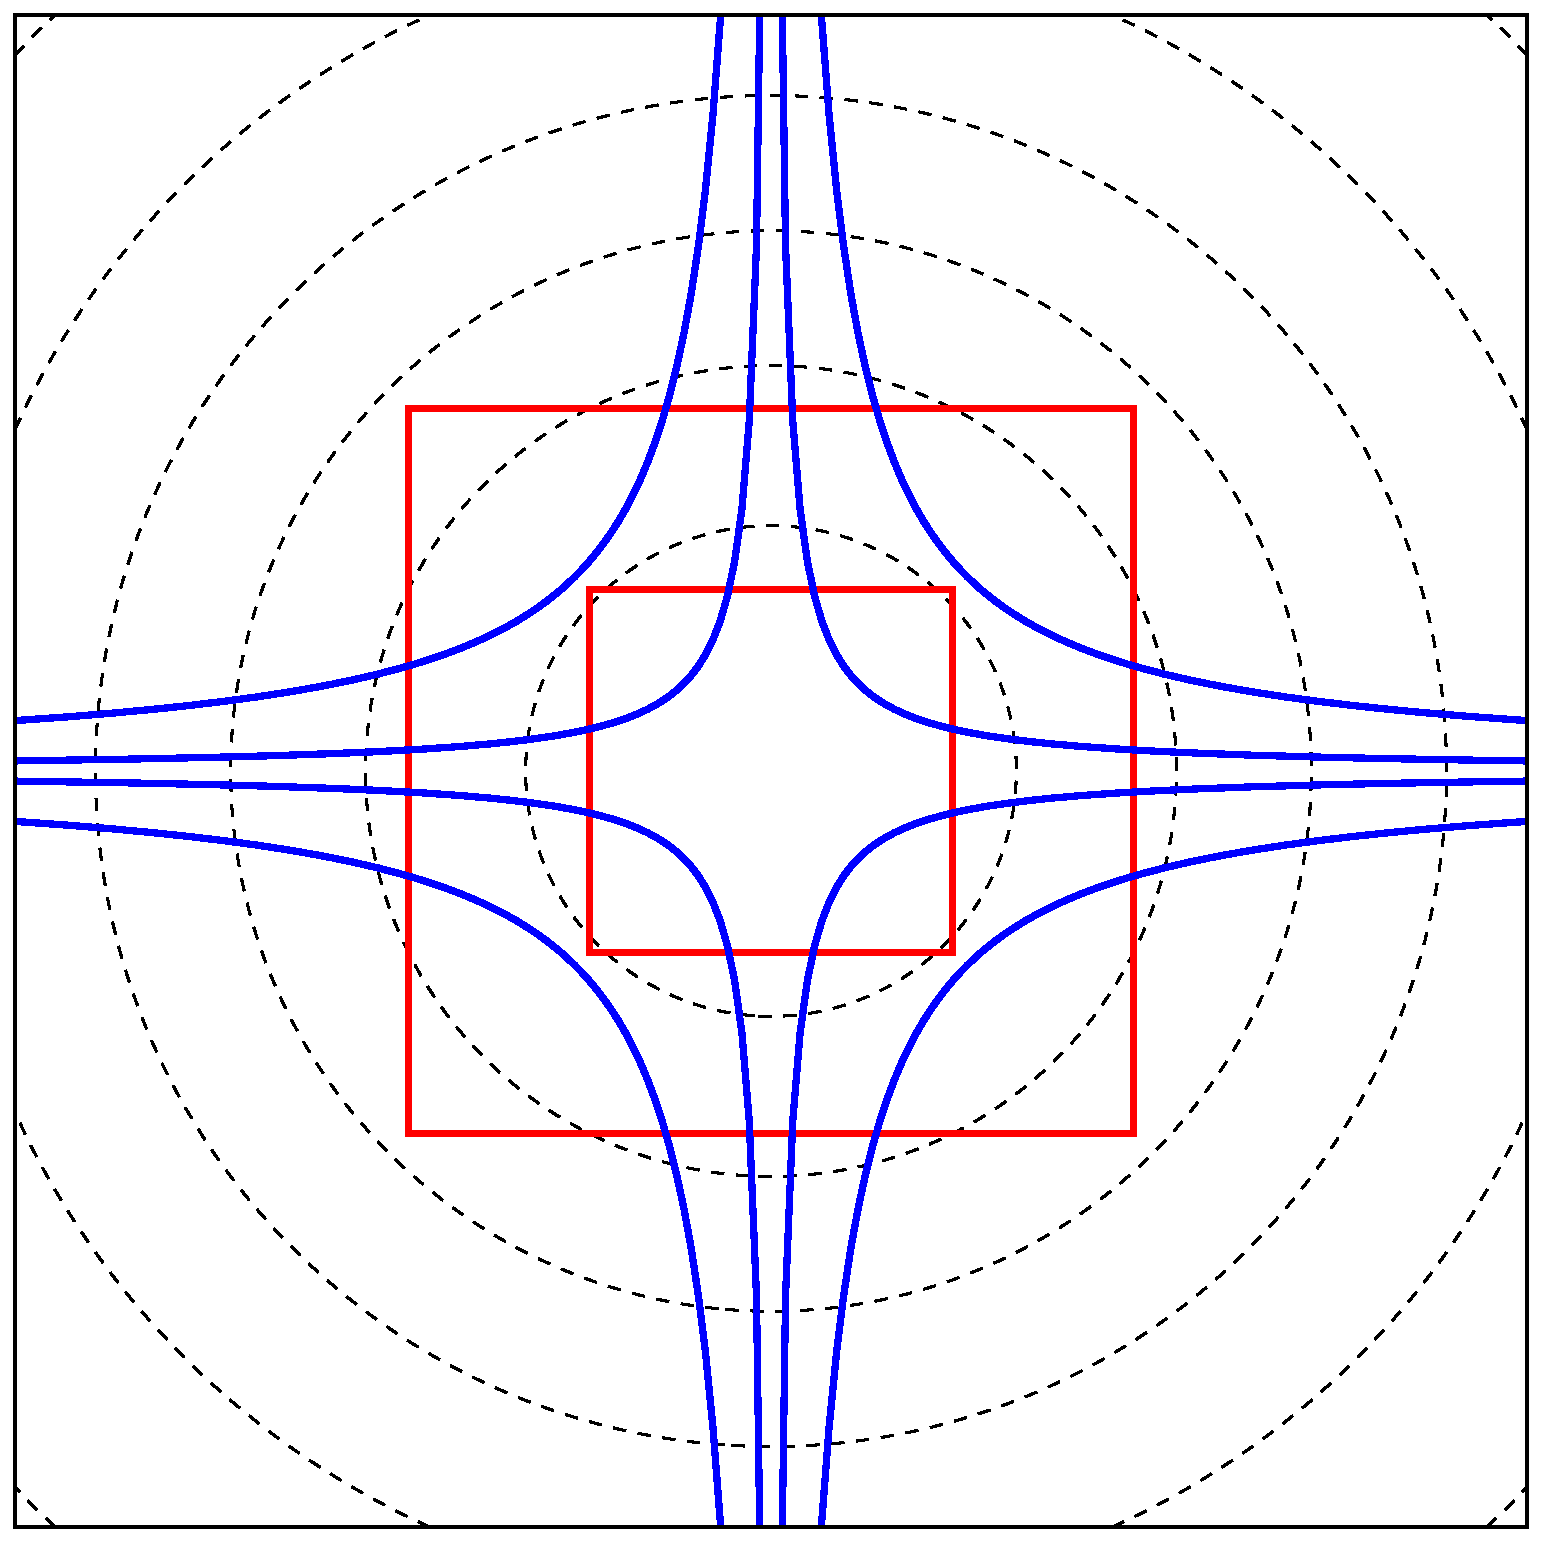
\includegraphics[width=4cm]{../figs/hcboltz/hcgauss}
    \caption{{\color{red}$\AFF$} and {\color{blue}$\cA_{Y=0}$} compared to the Gaussian spectrum.}
\end{figure}
\end{frame}

\begin{frame}{Hyperbolic cross vs. Full grid}
\[
    \sharp\AFF(N) = N^d, \qquad \sharp\cA_{Y=0}(N) = \cO(N \log^d N)
\] \\~\\

The sets $\cA_Y$ do not resolve Maxwellians very well, but could still work well for solutions far removed
from equilibrium. \\~\\

For observables, note that off-axis wavenumbers $\Bk$ are massless, momentum-less and energy-less. Evaluation
of these functionals require only on-axis modes, so
\[
    \eta(P_{\cA_Y(N)} f) = \eta(P_{\AFF(N)}f) \qquad \forall f, N \qquad \eta = \rho, \Bu, E
\]
\end{frame}

\begin{frame}{Hyperbolic cross vs. Full grid}
Evaluation of the collision operator requires the evaluation of
\[
    f = \sum_{\Bk\in\cA} f_\Bk \ee^{\ii\Bk\cdot\Bv}
    \implies
    \frac{\partial f_\Bk}{\partial t} = \sum_{\substack{\Bl,\Bm\in\cA \\ \Bl+\Bm=\Bk}} 
    \hat{\beta}(\Bl,\Bm) f_\Bl f_\Bm
\]
Which has expense on the order of the size of the set
\[
    c(\cA) = \left\{ (\Bl,\Bm) \in \cA^2 \;:\; \Bl+\Bm \in \cA \right\}.
\]
\begin{align*}
    \sharp c(\AFF(N)) &= \cO([\sharp\AFF(N)]^2) \\
    \sharp c(\cA_{Y=0}(N)) &= \cO([\sharp\cA_{Y=0}(N)]^{\nicefrac{15}{8}})
\end{align*}
Hyperbolic cross is slightly more efficient per DoF.
\end{frame}

\begin{frame}{Perturbation method}
Close to equilibrium, we can write $f = f^p + \mu$, with small $f^p$.
\[
    \frac{\partial f}{\partial t} = \frac{\partial f^p}{\partial t} = 
    \underbrace{Q(f^p,f^p)}_{\text{small}} +
    \underbrace{Q(\mu,f^p) + Q(f^p,\mu)}_{\text{linear}}
\]
{\bf Question:} Could we approximate $f^p$ with hyperbolic cross and avoid the near-equilibrium problem? \\~\\

\begin{overlayarea}{\textwidth}{0.3cm}
\only<2>{{\bf Answer:} Doesn't work much better than normal HC. Near equilibrium, the perturbations $f^p$ also
tend to be radially symmetric.}
\end{overlayarea}
\end{frame}

\begin{frame}
Solutions tend toward radial symmetry {\em before} they tend to equilibrium.
\begin{figure}
\centering
\begin{tikzpicture}[scale=0.6]
    \draw[line width=0.02cm, <-<] (0.2,0.4) .. controls (0.2,4) and (2,5.8) .. (5.6,5.8);
    \draw[line width=0.02cm, dashed] (0,0) -- (6,6);
    \draw[line width=0.02cm, ->] (-1,0) -- (6,0);
    \draw[line width=0.02cm, ->] (0,-1) -- (0,6);
    \node[below right,align=center,scale=0.6] at (0,0) {Radially\\symmetric};
    \node[below left,align=center,scale=0.6] at (6,0) {Radially\\asymmetric};
    \begin{scope}[cm={0,1,-1,0,(0,0)}, every node/.style={transform shape}]
        \node[above right,align=center] at (0,0) {Equilibrium};
        \node[above left,align=center] at (6,0) {Not\\equilibrium};
    \end{scope}
\end{tikzpicture}
\end{figure}
Some theoretical justification from the Landau equation, some numerical justification to come.
\end{frame}

\begin{frame}{Polar discretization}
If radially symmetric solutions are such a strong tendency, a polar discretization could be useful. \\~\\

In angle: 
\[
    \xi_\ell(\theta) = \ee^{\ii \ell \theta}
\]

In radius:
\begin{align*}
    \psi_{k,\beta}^\rmS(r) &= \ee^{-\nicefrac{r^2}{\beta}} \; L_k^{(0)}(r^2) \\
    \psi_{k,\beta}^\rmK(r) &= \frac{1}{\sqrt{k+1}} \ee^{-\nicefrac{r^2}{\beta}} \; r \; L_k^{(1)}(r^2)
\end{align*}
$L_k^{(\alpha)}$ is the generalized Laguerre polynomial of order $\alpha$, degree $k$.
\end{frame}

\begin{frame}{Laguerre polynomials}
Generalized Laguerre polynomials are orthogonal on $[0,\infty)$ with respect to the measure
$e^{-x}x^{\alpha}\dd x$:
\[
    \int_0^\infty L^{(\alpha)}_k L^{(\alpha)}_\ell \ee^{-x}x^\alpha \dd x 
    = \binom{k+\alpha}{k} \Gamma(\alpha + 1) \delta_{k,\ell}.
\]
In particular, $\psi_{k,\beta}^\rmS$ and $\psi_{k,\beta}^\rmK$ are orthogonal with respect to the measure
\[
    e^{-(1-\nicefrac{2}{\beta})r^2} r \dd r
\]
which fits with the 2D volume element in polar coordinates.
\end{frame}

\pgfplotstableread{radial1.txt} \radialdataone
\pgfplotstableread{radial2.txt} \radialdatatwo

\begin{frame}
\frametitle{Radial basis functions}
\begin{centering}
\begin{equation*}
    \beta=1
\end{equation*}
\begin{tikzpicture}[xscale=0.77, yscale=0.4]
    \begin{axis}
    [
        xmin = 0,
        xmax = 3,
        ymin = -0.34,
        ymax = 1,
        axis x line* = middle,
        axis y line* = left,
        ticks = none,
    ]
        \addplot[color=yellow, mark=none, line width=1] table[y=y0] from \radialdataone;
        \addplot[color=orange, mark=none, line width=1] table[y=y2] from \radialdataone;
        \addplot[color=red, mark=none, line width=1] table[y=y4] from \radialdataone;
        \addplot[color=magenta, mark=none, line width=1] table[y=y6] from \radialdataone;
        \addplot[color=violet, mark=none, line width=1] table[y=y8] from \radialdataone;
        \addplot[color=blue, mark=none, line width=1] table[y=y10] from \radialdataone;
        \addplot[color=cyan, mark=none, line width=1] table[y=y12] from \radialdataone;
        \addplot[color=green, mark=none, line width=1] table[y=y14] from \radialdataone;
    \end{axis}
\end{tikzpicture}
\begin{tikzpicture}[xscale=0.77, yscale=0.4]
    \begin{axis}
    [
        xmin = 0,
        xmax = 3,
        ymin = -0.25,
        ymax = 0.56,
        axis x line* = middle,
        axis y line* = left,
        ticks = none,
    ]
        \addplot[color=yellow, mark=none, line width=1] table[y=y1] from \radialdataone;
        \addplot[color=orange, mark=none, line width=1] table[y=y3] from \radialdataone;
        \addplot[color=red, mark=none, line width=1] table[y=y5] from \radialdataone;
        \addplot[color=magenta, mark=none, line width=1] table[y=y7] from \radialdataone;
        \addplot[color=violet, mark=none, line width=1] table[y=y9] from \radialdataone;
        \addplot[color=blue, mark=none, line width=1] table[y=y11] from \radialdataone;
        \addplot[color=cyan, mark=none, line width=1] table[y=y13] from \radialdataone;
        \addplot[color=green, mark=none, line width=1] table[y=y15] from \radialdataone;
    \end{axis}
\end{tikzpicture}
\begin{equation*}
    \beta=2
\end{equation*}
\begin{tikzpicture}[xscale=0.77, yscale=0.4]
    \begin{axis}
    [
        xmin = 0,
        xmax = 7,
        ymin = -0.45,
        ymax = 1,
        axis x line* = middle,
        axis y line* = left,
        ticks = none,
    ]
        \addplot[color=yellow, mark=none, line width=1] table[y=y0] from \radialdatatwo;
        \addplot[color=orange, mark=none, line width=1] table[y=y2] from \radialdatatwo;
        \addplot[color=red, mark=none, line width=1] table[y=y4] from \radialdatatwo;
        \addplot[color=magenta, mark=none, line width=1] table[y=y6] from \radialdatatwo;
        \addplot[color=violet, mark=none, line width=1] table[y=y8] from \radialdatatwo;
        \addplot[color=blue, mark=none, line width=1] table[y=y10] from \radialdatatwo;
        \addplot[color=cyan, mark=none, line width=1] table[y=y12] from \radialdatatwo;
        \addplot[color=green, mark=none, line width=1] table[y=y14] from \radialdatatwo;
    \end{axis}
\end{tikzpicture}
\begin{tikzpicture}[xscale=0.77, yscale=0.4]
    \begin{axis}
    [
        xmin = 0,
        xmax = 7,
        ymin = -0.40,
        ymax = 0.61,
        axis x line* = middle,
        axis y line* = left,
        ticks = none,
    ]
        \addplot[color=yellow, mark=none, line width=1] table[y=y1] from \radialdatatwo;
        \addplot[color=orange, mark=none, line width=1] table[y=y3] from \radialdatatwo;
        \addplot[color=red, mark=none, line width=1] table[y=y5] from \radialdatatwo;
        \addplot[color=magenta, mark=none, line width=1] table[y=y7] from \radialdatatwo;
        \addplot[color=violet, mark=none, line width=1] table[y=y9] from \radialdatatwo;
        \addplot[color=blue, mark=none, line width=1] table[y=y11] from \radialdatatwo;
        \addplot[color=cyan, mark=none, line width=1] table[y=y13] from \radialdatatwo;
        \addplot[color=green, mark=none, line width=1] table[y=y15] from \radialdatatwo;
    \end{axis}
\end{tikzpicture}
\end{centering}
\end{frame}

\begin{frame}{Polar Laguerre function space}
Renumbering for convenience
\begin{gather*}
    \varphi_k = \begin{cases} \psi^\rmS_{\nicefrac{k}{2}}, & k \equiv 0 \;(\Mod 2), \\
                              \psi^\rmK_{\nicefrac{(k-1)}{2}}, & k \equiv 1 \;(\Mod 2)
                \end{cases}
\end{gather*}
\[
    V_\beta(K,L) = \spann \left\{ \varphi_k^{(\beta)} \xi_\ell \;:\; 
    (0,-L) \leq (k,\ell) < (K,L),\; k\equiv\ell \;(\Mod 2) \right\}
\]
\begin{theorem}[$\beta$-orthogonality]
    Let $\mu(r) = \ee^{-r^2}$. Then
    \begin{align*}
        \langle \varphi_{k_1} \xi_{\ell_1}, \varphi_{k_2} \xi_{\ell_2} \rangle_{L^2(\bbR^2,\beta)}
        &= \int \mu^{1-\nicefrac{2}{\beta}} \varphi_{k_1} \xi_{\ell_1} \varphi_{k_2} \xi_{-\ell_2} \\
        &= \pi \; \delta_{k_1,k_2} \; \delta_{\ell_1,\ell_2}.
    \end{align*}
\end{theorem}
\end{frame}

\begin{frame}{Choosing $\beta$}
\begin{theorem}[Stability w.r.t. observables]
    \begin{align*}
        \rho(\xi_0\psi^\rmS_k) &= \beta\pi{\color{red}(1-\beta)^k}, \\
        (\Bu\rho)(\xi_{\pm1}\psi^\rmK_k) &= \frac{\beta^2\pi}{2}\begin{pmatrix}1\\\pm1\end{pmatrix}
        \sqrt{k+1} {\color{red}(1-\beta)^k}, \\
        (E\rho)(\xi_0\psi^\rmS_k) &= \begin{cases} \beta^2\pi[1-(k+1)\beta]
                                                    {\color{red}(1-\beta)^{k-1}}, & k>0 \\
                                                    \beta^2\pi, & k=0. \end{cases}
    \end{align*}
\end{theorem}
\end{frame}

\begin{frame}{Choosing $\beta$}
Corollary:
\begin{itemize}
    \item[\good] For $0<\beta<2$, observables are $\cO(|\beta-1|^k)$.
    \item[\good\good] For $\beta=1$, observables become zero $\implies$ conservation.
    \item[\bad] For $\beta=2$, observables are $\cO(k)$.
    \item[\bad\bad] For $\beta>2$, observables are $\cO(|\beta-1|^k)$.
\end{itemize}
Other considerations:
\begin{itemize}[label=\ding{221}]
    \item Higher $\beta$ usually gives better convergence (both norms).
    \item $\beta>2$ gives unbounded basis functions.
    \item For $\beta=2$, we have orthogonality w.r.t. Lebesgue measure.
\end{itemize}
We have run experiments with $\beta=1,2$.
\end{frame}

\begin{frame}{Equilibrium and conformity}
Function space contains
\begin{equation*}
    \varphi_0 \xi_0 = \ee^{-\nicefrac{r^2}{\beta}} = \mu^{\nicefrac{1}{\beta}},
\end{equation*}
which is an equilibrium solution with
\begin{equation} \label{eq:conf}
    \rho = \beta\pi, \qquad \Bu=\Bzero, \qquad T = \frac{\beta}{2}.
\end{equation}
\begin{definition}[$\beta$-conformity]
    A function $f$ is $\beta$-conforming if it satisfies \eqref{eq:conf}.
\end{definition}
\end{frame}

\begin{frame}{Conformity}
\begin{theorem}
    Assume $f(t,\Bv)$ is a solution with mass, momentum and temperature $\rho$, $\Bu$ and $T$. Let
    \begin{equation*}
        \gamma = \sqrt{\frac{2T}{\beta}}, \qquad
        \alpha = \frac{2\pi T}{\rho}, \qquad
        \eta = \frac{\alpha}{\gamma^{\lambda+2}}
    \end{equation*}
    and define $g(t,\Bv) = \alpha f(\eta t, \gamma \Bv + \Bu)$. Then $g$ is a $\beta$-conforming solution.
\end{theorem}
\end{frame}

\begin{frame}{Evaluating collisions}
\begin{equation*}
    f = \sum_{k,\ell} F_k^\ell\varphi_k\xi_\ell \implies
    Q(f,f) = \sum_{k,\ell} 
    \left( \sum S_{k_1,k_2,\ell_1,\ell_2}^{k,\ell} F_{k_1}^{\ell_1} F_{k_2}^{\ell_2} \right) 
    \varphi_k\xi_\ell
\end{equation*}
where
\begin{equation*}
    S_{k_1,k_2,\ell_1,\ell_2}^{k,\ell} = \frac{1}{\pi} \left\langle 
    Q(\varphi_{k_1}\xi_{\ell_1}, \varphi_{k_2}\xi_{\ell_2}), \varphi_k \xi_\ell
    \right\rangle_{L^2(\bbR^2,\beta)}
\end{equation*}
\begin{itemize}
    \item[\bad] Expensive.
    \item[\good] $S_{k_1,k_2,\ell_1,\ell_2}^{k,\ell} = 0$ 
        unless $\ell=\ell_1+\ell_2$. We're ``only'' one order behind Fourier:
        $\cO(N^{2d+1})$ vs. $\cO(N^{2d})$.
    \item[\good] The solution space should shrink significantly for large times.
\end{itemize}
\end{frame}

\begin{frame}{The number crunching (loss part)}
\begin{equation*}
    S^{-} = \frac{1}{\pi} 
    \int_{\Bv} \mu^{1-\nicefrac{2}{\beta}} \varphi_{k_1} \varphi_k \xi_{\ell_1} \xi_{-\ell}
    \int_{\Bv_\ast} \varphi_{k_2} \xi_{\ell_2}
    \int_\Bsigma B
\end{equation*}
The inner integral couples $\Bv$ and $\Bv_\ast$,
\begin{equation*}
    \cI^-(\Bv,\Bv_\ast) = |\Bv-\Bv_\ast|^\lambda 
    \underbrace{\int_\Bsigma b(\cos\theta)}_{\text{const.}}
\end{equation*}
If $B\equiv\text{const.}$ (i.e. $\lambda=0$, Maxwellian kernel):
\begin{equation*}
    S^{-} = \delta_{k,k_1} \; \delta_{\ell,\ell_1} \; \delta_{0,\ell_2} \; \rho(\varphi_{k_2}).
\end{equation*}
\end{frame}

\begin{frame}{The number crunching (gain part)}
\begin{equation*}
    S^{+} = \frac{1}{\pi} 
    \int_{\Bv} \varphi_{k_1} \xi_{\ell_1}
    \int_{\Bv_\ast} \varphi_{k_2} \xi_{\ell_2}
    \int_\Bsigma B \mu^{1-\nicefrac{2}{\beta}} \varphi_k \xi_{-\ell}
\end{equation*}
The inner integral is now (assuming $b\equiv\text{const.}$)
\begin{align*}
    \cI^+(\Bv,\Bv_\ast) &= |\Bv-\Bv_\ast|^\lambda b
    \int_\Bsigma \left[\mu^{1-\nicefrac{2}{\beta}} \varphi_k \xi_{-\ell} \right] (\Bv') \\
    &= |\Bv-\Bv_\ast|^\lambda b \; \xi_{-\ell}(\Bv+\Bv_\ast)
    \int_\Bsigma \left[\mu^{1-\nicefrac{2}{\beta}} \varphi_k \xi_{-\ell} \right] (\Bw')
\end{align*}
after substituting $\Bv' = \ee^{\ii \arg(\Bv+\Bv_\ast)} \Bw'$. The integral only depends on two real
parameters!
\end{frame}

\begin{frame}
\centering
\begin{tikzpicture}
    \coordinate[label={[label distance=1cm]45:$\Bv'$}] (before) at (40:5);
    \coordinate[label={[label distance=1cm]15:$\Bw'$}] (after) at (0:5);
    \coordinate[label={0:$\arg(\Bv+\Bv_\ast)$}] (angle) at (25:1);
    \draw[densely dotted, <-, line width=1] (0:5) arc (0:40:5);
    \draw[line width=1] (0:1) arc (0:40:1);
    \draw[densely dotted, line width=1] (0,0) -- (before);
    \draw[line width=1] (before) circle (1);
    \draw[line width=1] (after) circle (1);
    \draw[line width=1,->] (-1,0) -- (8,0);
    \draw[line width=1,->] (0,-1) -- (0,4);
\end{tikzpicture}
\end{frame}

\begin{frame}{Convergence}
\begin{theorem}
    Assume $f_0 \in L^\infty \cap H^{u,v}_{\mathsf{mix}}$ is nonnegative and that 
    \[
        \|f_0 - P_{\cA_Y} f_0\|_{L^\infty(\cD_L)} \xrightarrow{N\to\infty} 0
    \]
    Then, for all $N$ sufficiently large
    \begin{itemize}[label=\ding{221}]
        \item There is a unique solution $f_{\cA_Y} \in H^{u,v}_{\mathsf{mix}}$ on $[0,T_{\mathsf{max}}]$
            uniformly bounded in $L^1$.
        \item The negative part of $f_{\cA_Y}$ is bounded pointwise by some $\eta(N)$ that vanishes as
            $N\to\infty$.
        \item With $f_R$ the solution to the truncated continuous equation
            \[
                \|f_R - f_{\cA_Y}\|_{H^s} \lesssim \left( C_{u,v,s}(L) + \|f_0\|_{H^{u,v}_{\mathsf{mix}}} \right)
                N^r \exp\left[ \gamma L^{2\lambda^{(+)} + \nicefrac{d}{2}} C_s(L) t \right]
            \]
    \end{itemize}
\end{theorem}
\end{frame}

\begin{frame}{Convergence}
The rate of convergence $r$ in $N$ is
\[
    r = \begin{cases}
        s-u-v+(Yu-s+v)\frac{d-1}{d-Y}, & Y \geq \frac{s-v}{u}, \\
        s-u-v, & Y < \frac{s-v}{u}.
    \end{cases}
\]
The proof can be extended to $\|f_{\cA_Y}-f\|$ provided some decay of $f$ and $f_R$ are assumed. \\~\\

Similar estimates for the polar scheme are not available, and the proofs are not easily generalized (in
particular, a strict positivity result for positive times is needed). \\~\\

Under suitable assumptions on the decay and analyticity of $f$, stationary approximation in $V_\beta(K,L)$ is
$\cO(\ee^{-\sqrt{K}} + \ee^{-L})$.
\end{frame}

\begin{frame}{Verification (BKW)}
The only known nontrivial analytic solution:
\[
    f(t,v) = (2\pi s)^{-d/2} \exp\left(-\frac{|\Bv|^2}{2s}\right)
            \left(1-\frac{1-s}{2s} \left(d-\frac{|\Bv|^2}{s}\right)\right)
\]
where 
\[
    s = s(t) = 1 - e^{-\zeta(t+t_0)},
\]
and $B=\text{const.}=\nicefrac{1}{2\pi}$ for $d=2$ $\implies \zeta=\nicefrac{1}{8}$.
\end{frame}

\begin{frame}{BKW: Fourier near equilibrium}
\centering
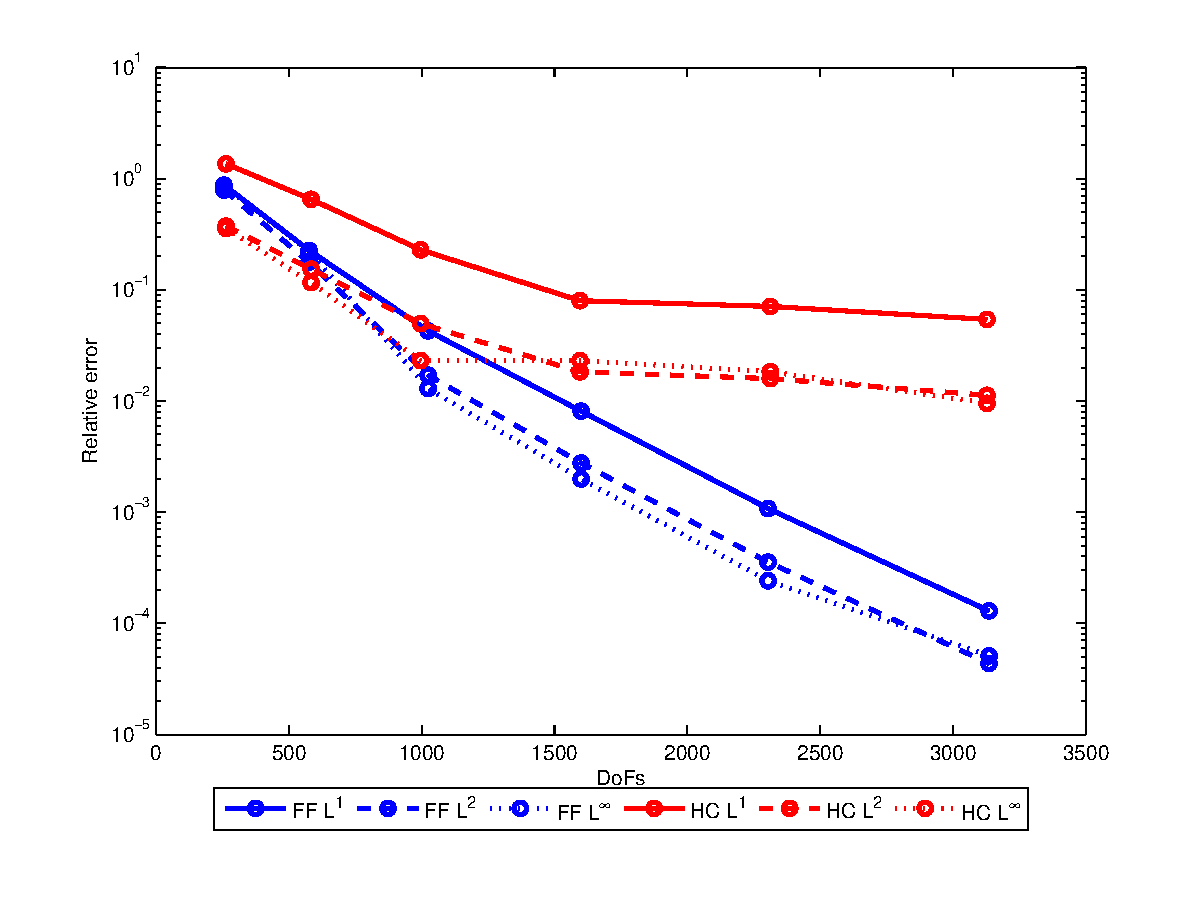
\includegraphics[width=11cm]{../figs/hcboltz/bkw5-1}
\end{frame}

\begin{frame}{BKW: Fourier w.r.t. time}
\centering
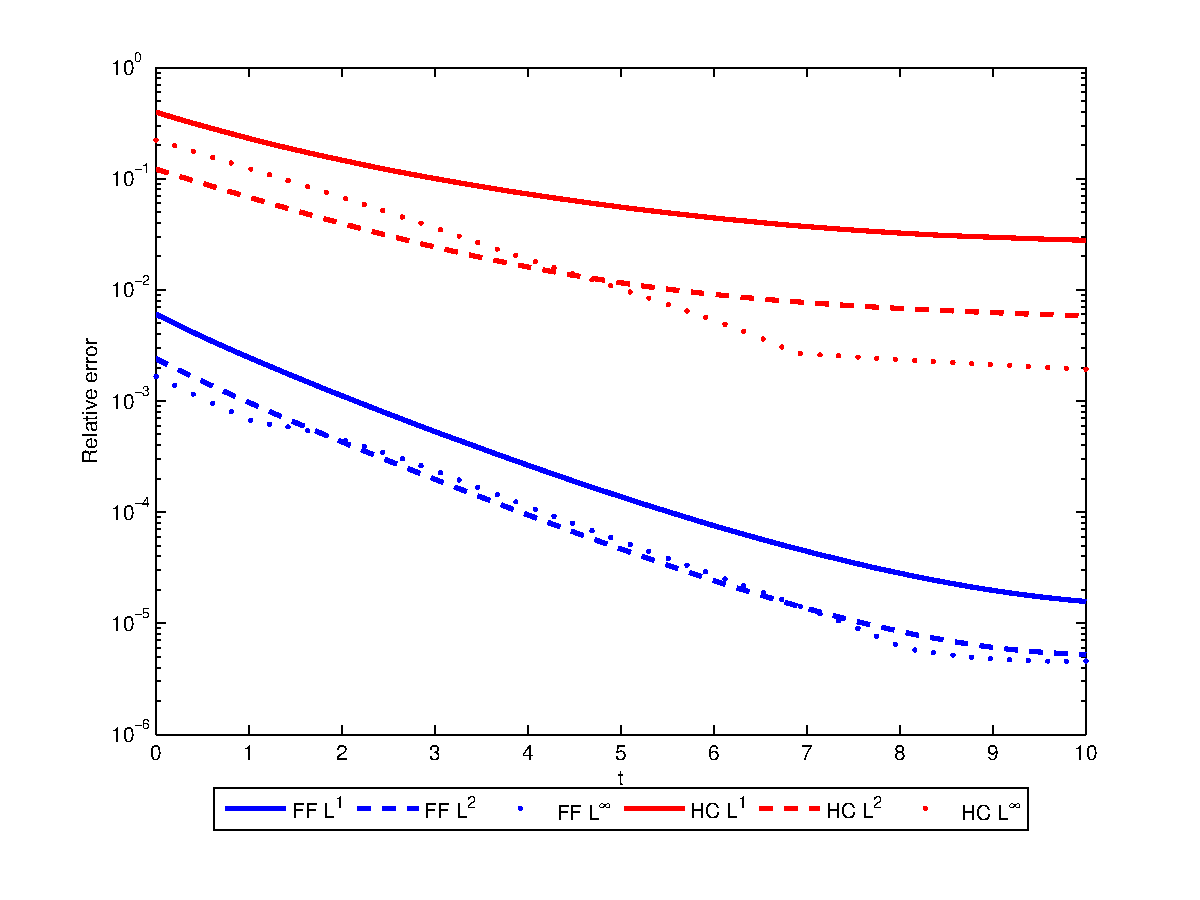
\includegraphics[width=11cm]{../figs/hcboltz/bkwtime}
\end{frame}

\begin{frame}{BKW: Polar}
\centering
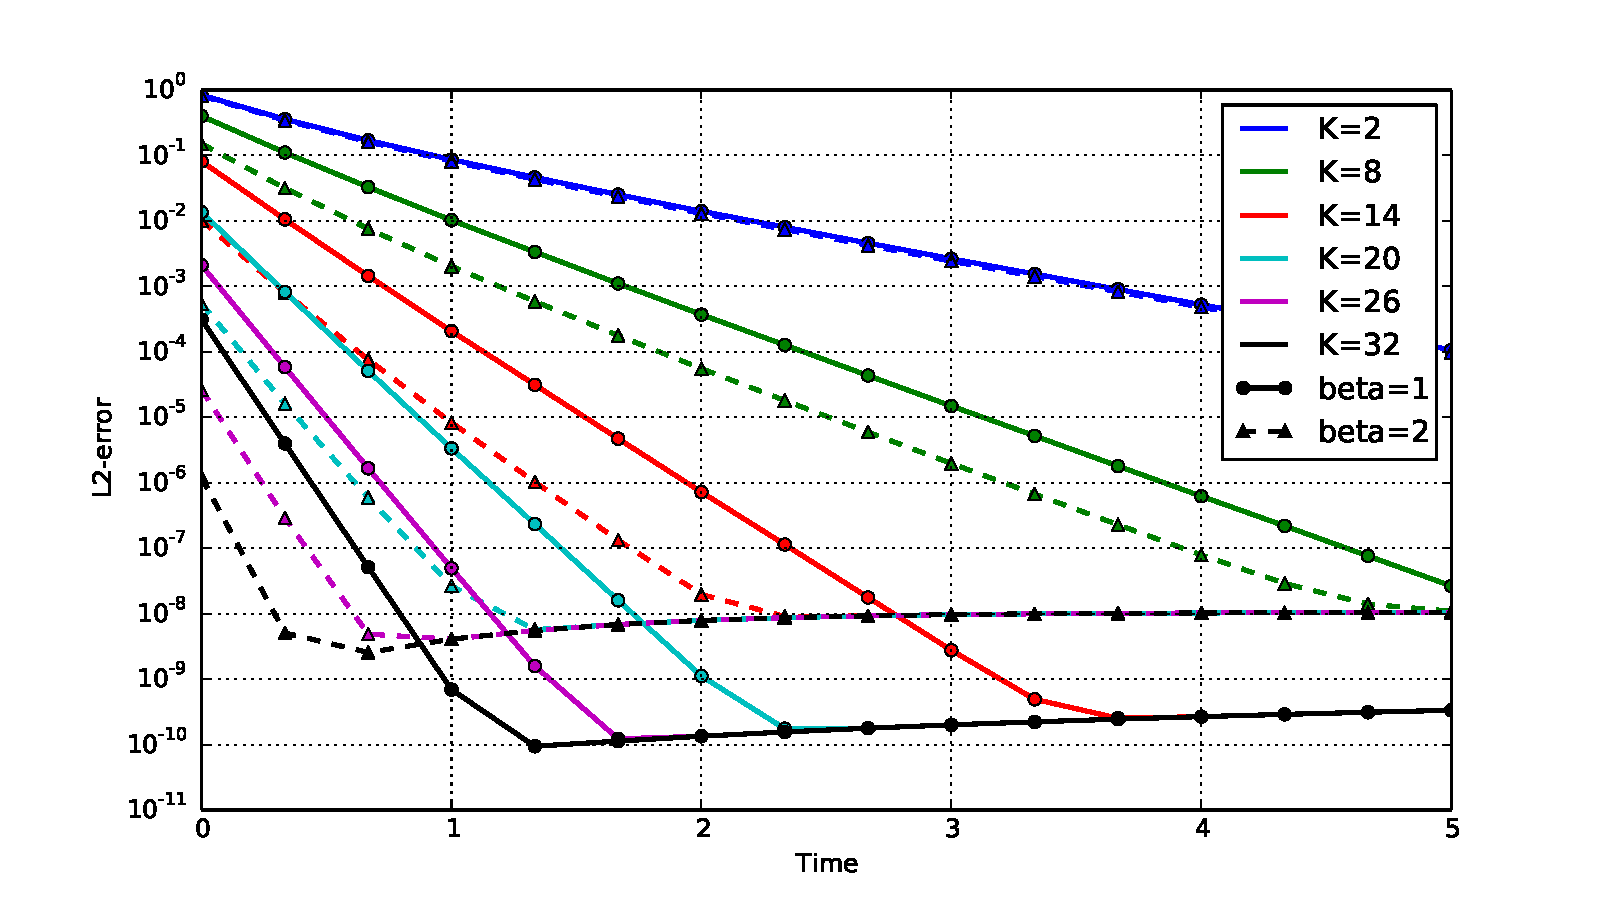
\includegraphics[width=11cm]{../figs/polboltz/bkw}
\end{frame}

\begin{frame}{BKW: Polar}
\centering
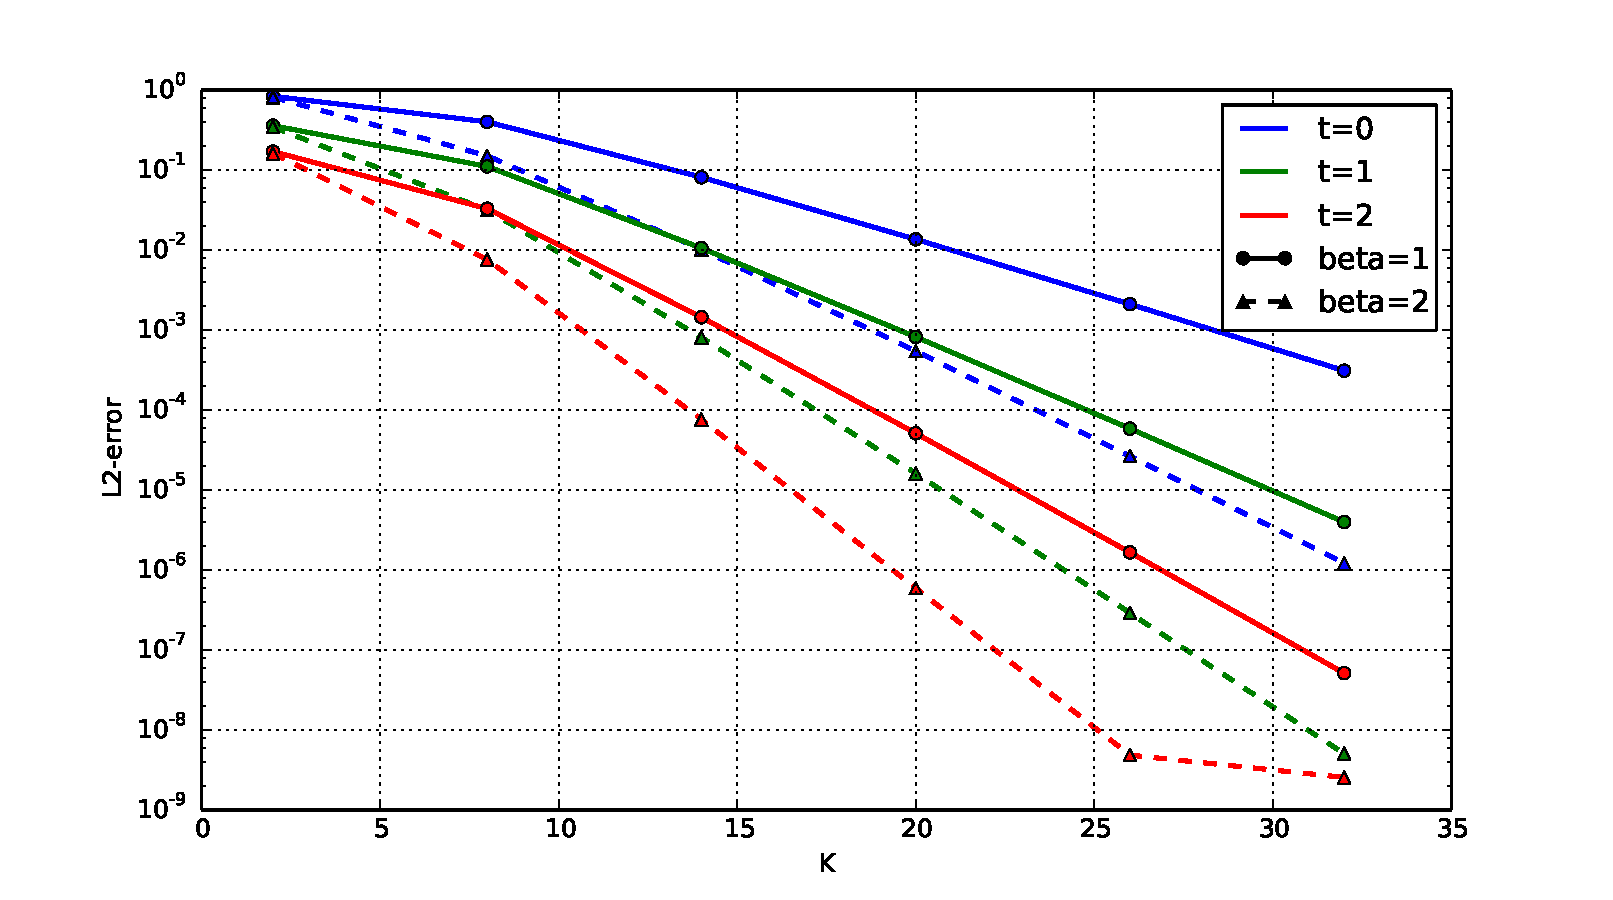
\includegraphics[width=11cm]{../figs/polboltz/bkw-flip}
\end{frame}

\begin{frame}{CS: Fourier}
A case where the HC works well.
\[
    f_0(\Bv) = \left[(1+\sin(sv_x))e^{-sv_x^2} + 
            (1+\sin(sv_y))e^{-sv_y^2}\right] e^{-2\|\Bv\|^2}
\]
with $s=10$. Approximately a sum of two elongated Gaussians. \\~\\

\centering
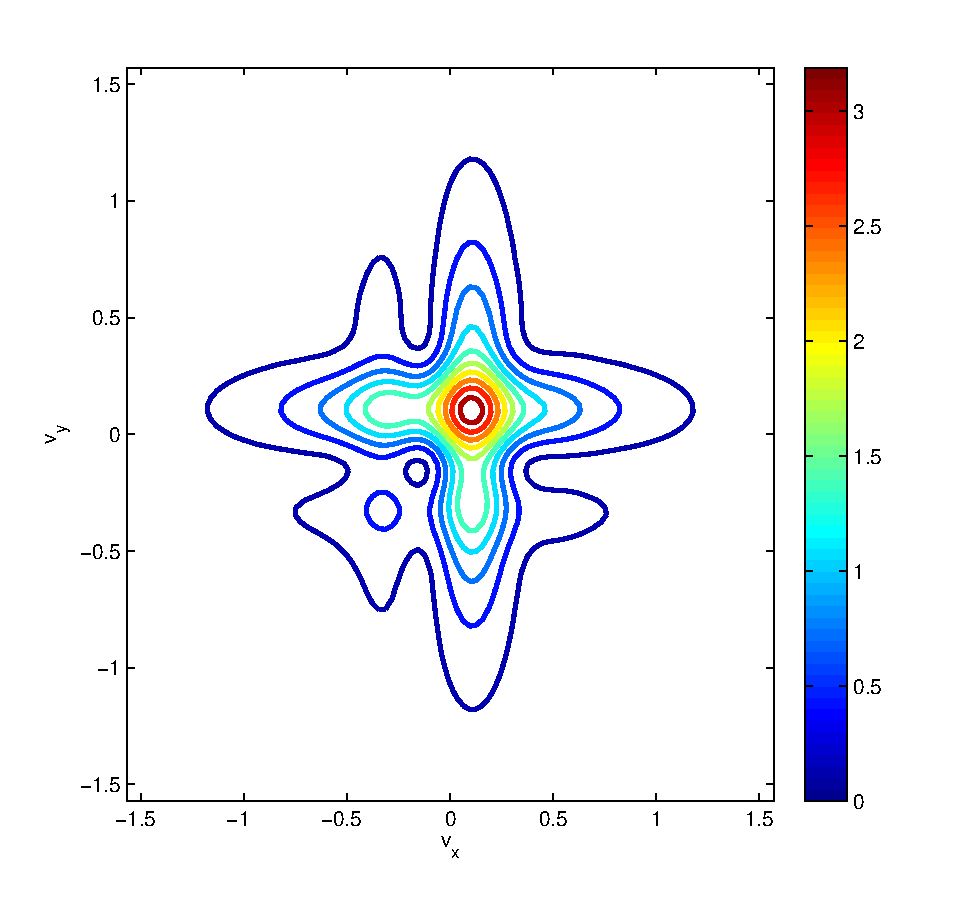
\includegraphics[width=3.87cm,height=3cm]{../figs/hcboltz/crossed-1}
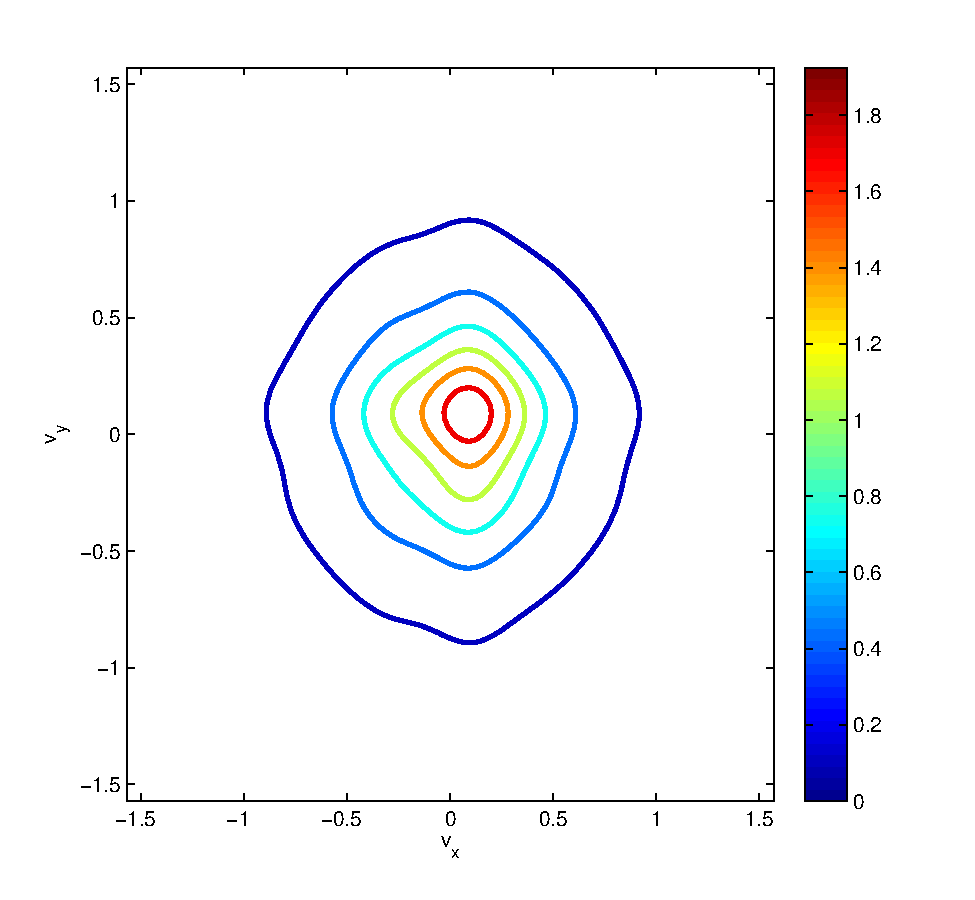
\includegraphics[width=3.87cm,height=3cm]{../figs/hcboltz/crossed-3}
\end{frame}

\begin{frame}{CS: Fourier, errors}
\centering
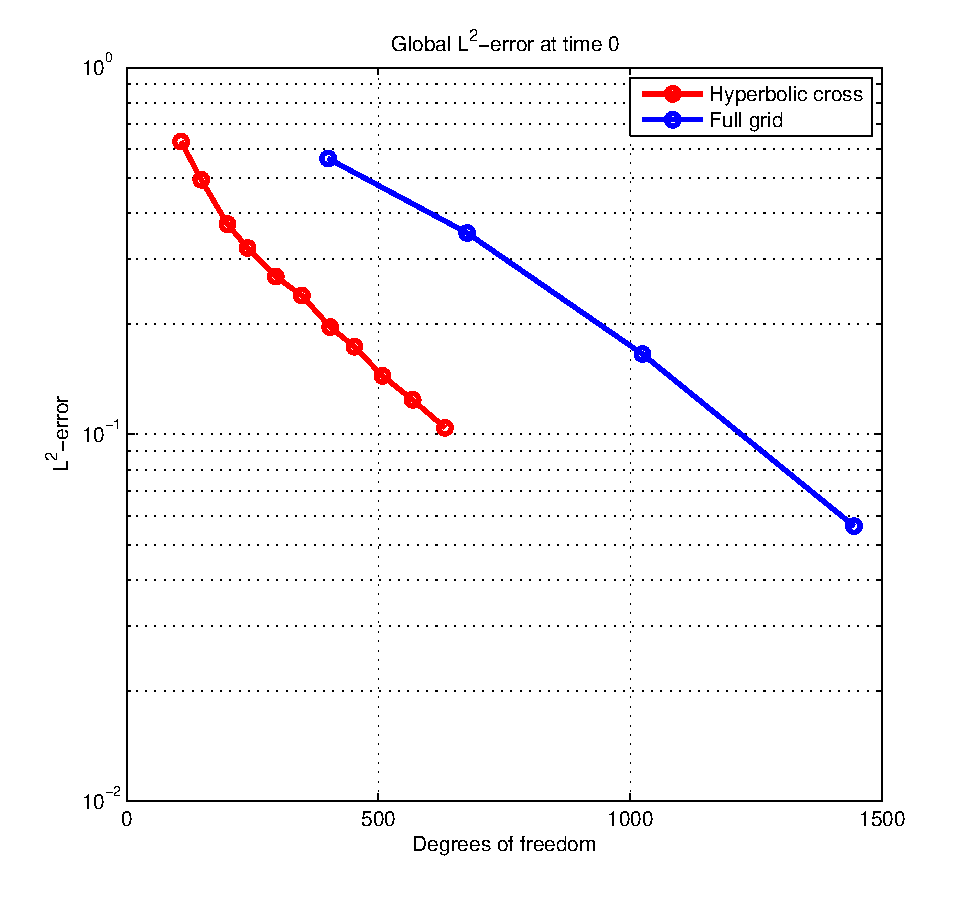
\includegraphics[width=4.0cm]{../figs/hcboltz/hc1-l2-1}
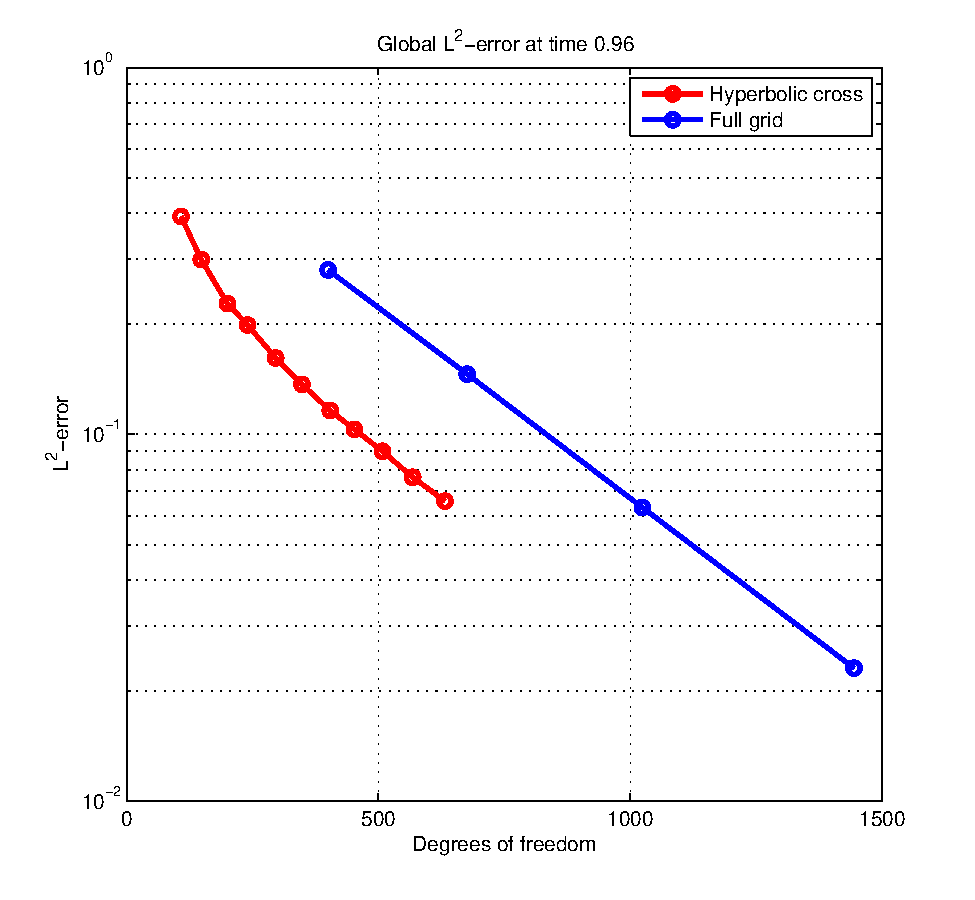
\includegraphics[width=4.0cm]{../figs/hcboltz/hc1-l2-2} \\
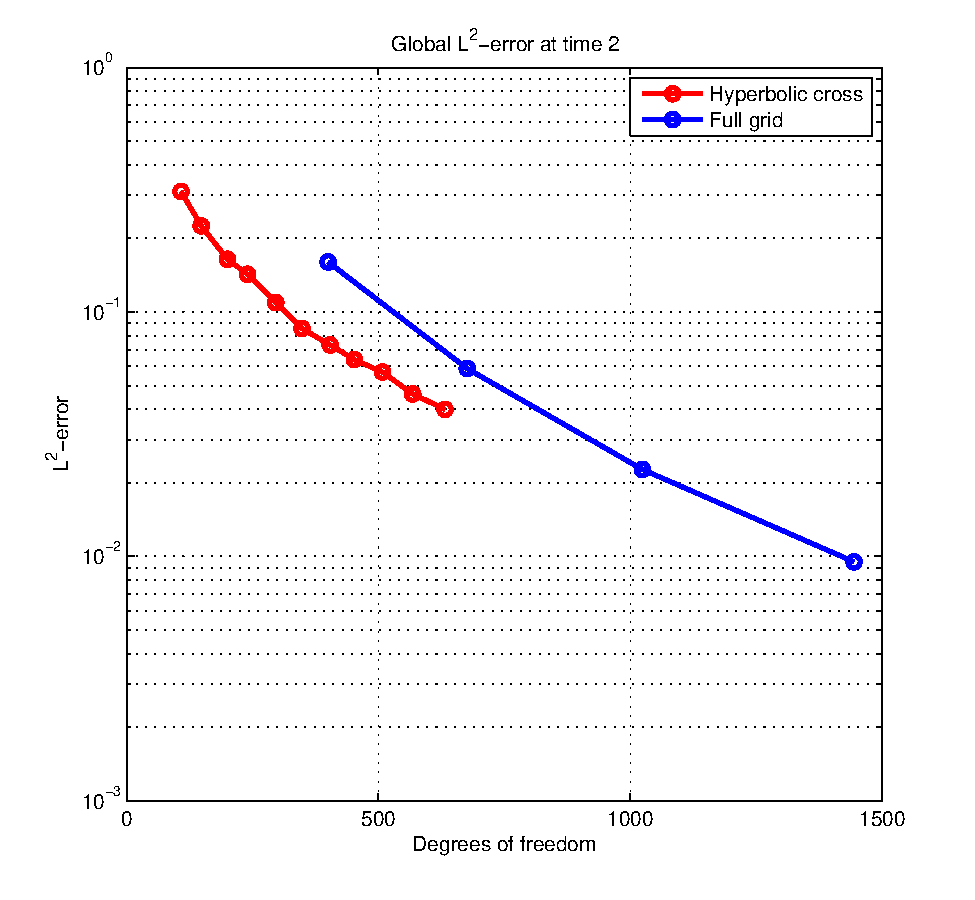
\includegraphics[width=4.0cm]{../figs/hcboltz/hc1-l2-3}
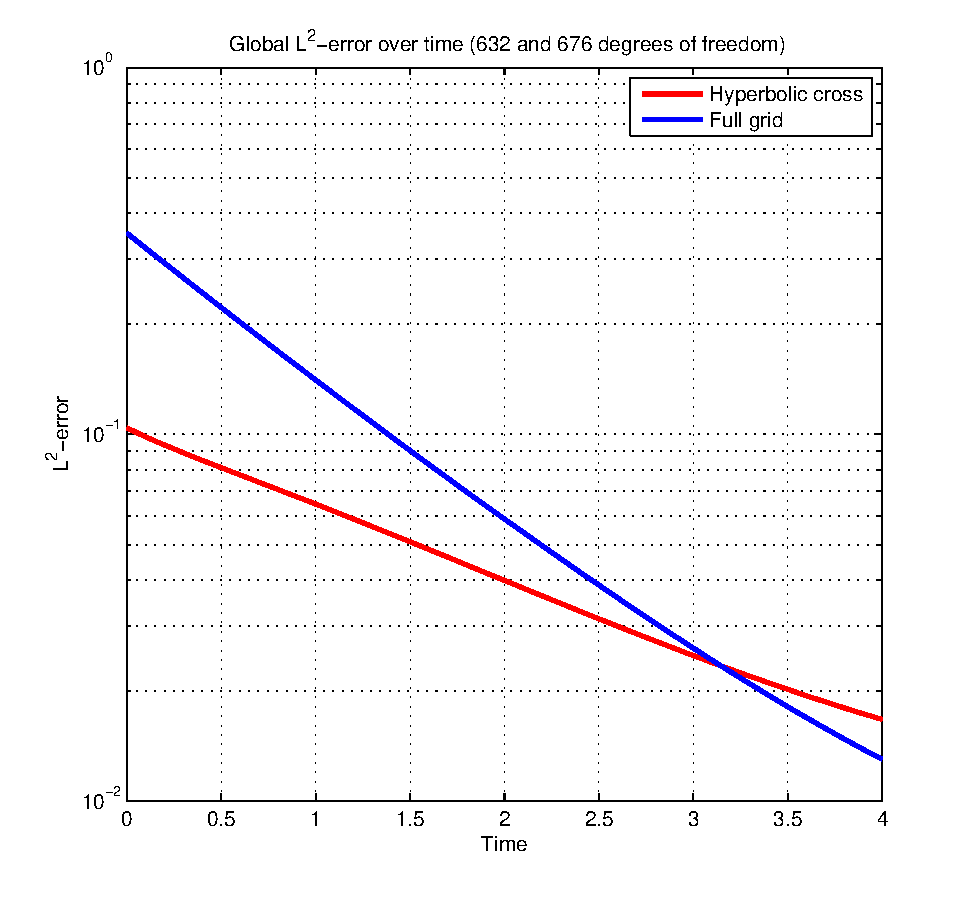
\includegraphics[width=4.0cm]{../figs/hcboltz/hc1-l2-time}
\end{frame}

\begin{frame}{CS: Polar}
2-conforming sum of elongated Gaussians:
\begin{align*}
    \eta(c,v,w) &= \exp\left[-g(S(v-c)^2 + (w-c)^2)\right] \\
    f_0(\Bv) &= \alpha\left( \eta(c,v_x,v_y) + \eta(-c,v_y,v_x) \right)
\end{align*}
\begin{gather*}
    \delta = 4R^2+\frac{1}{S}+1, \qquad
    \alpha = \frac{\delta}{4}\sqrt{S}, \qquad
    g = \frac{\delta}{4}, \qquad
    c = \frac{R}{\sqrt{g}}, \\
    S=3, \qquad R=1
\end{gather*}
\end{frame}

\begin{frame}{CS: Polar, error in observables}
\centering
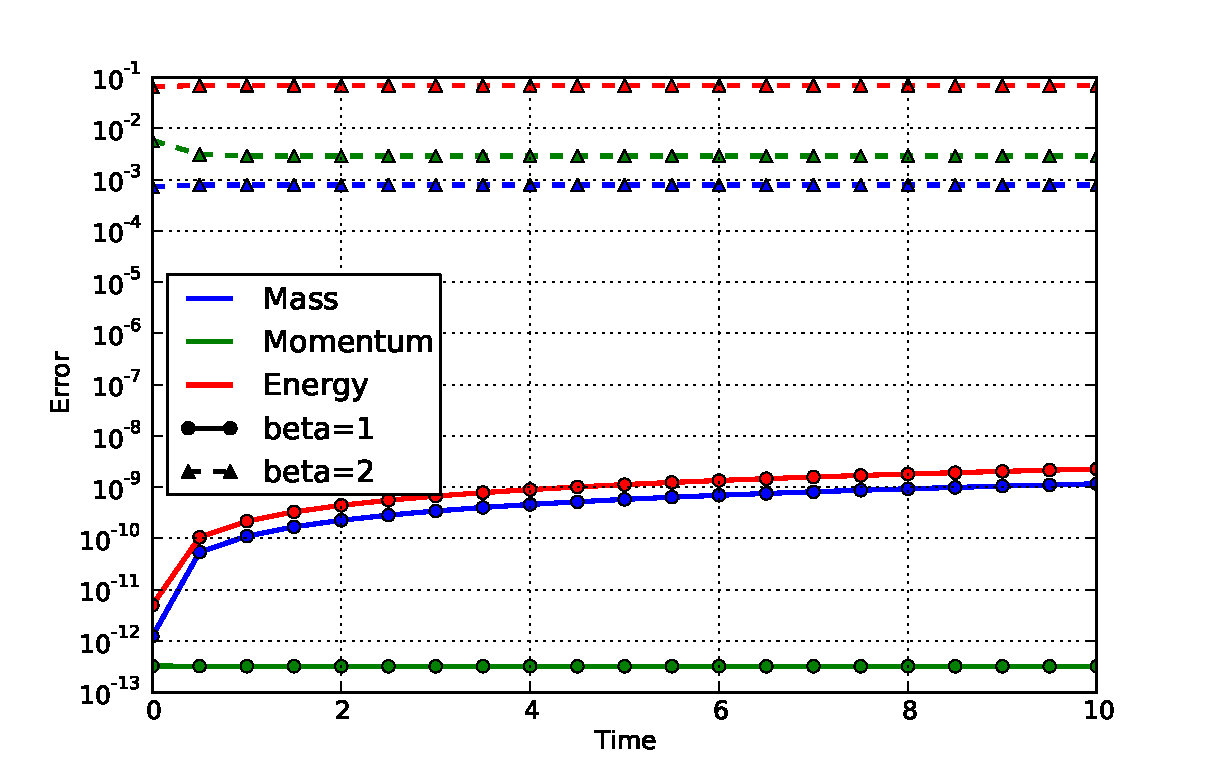
\includegraphics[width=11cm]{../figs/polboltz/scrossed-obs}
\end{frame}

\begin{frame}{CS: Polar, power contribution}
\centering
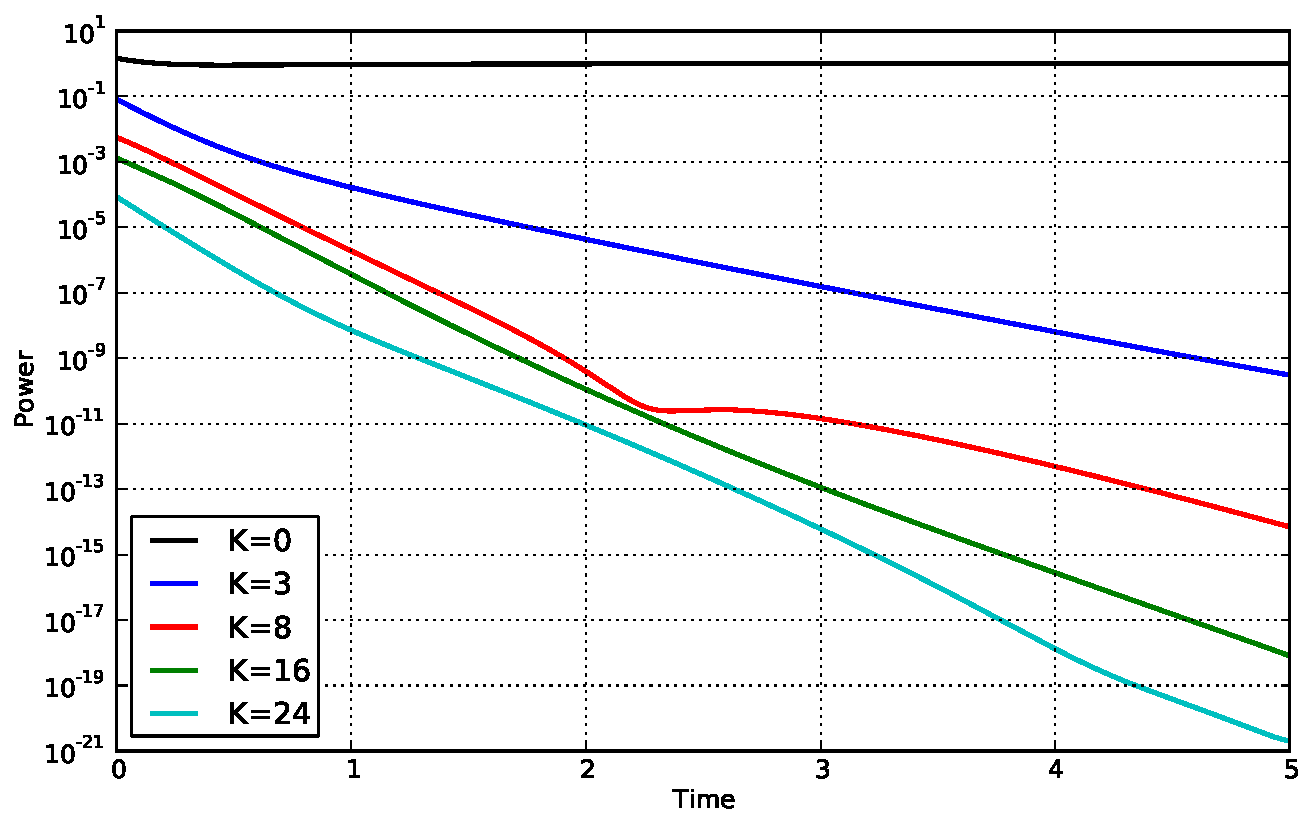
\includegraphics[width=11cm]{../figs/polboltz/power}
\end{frame}

\begin{frame}{CS: Polar, effort per timestep}
\centering
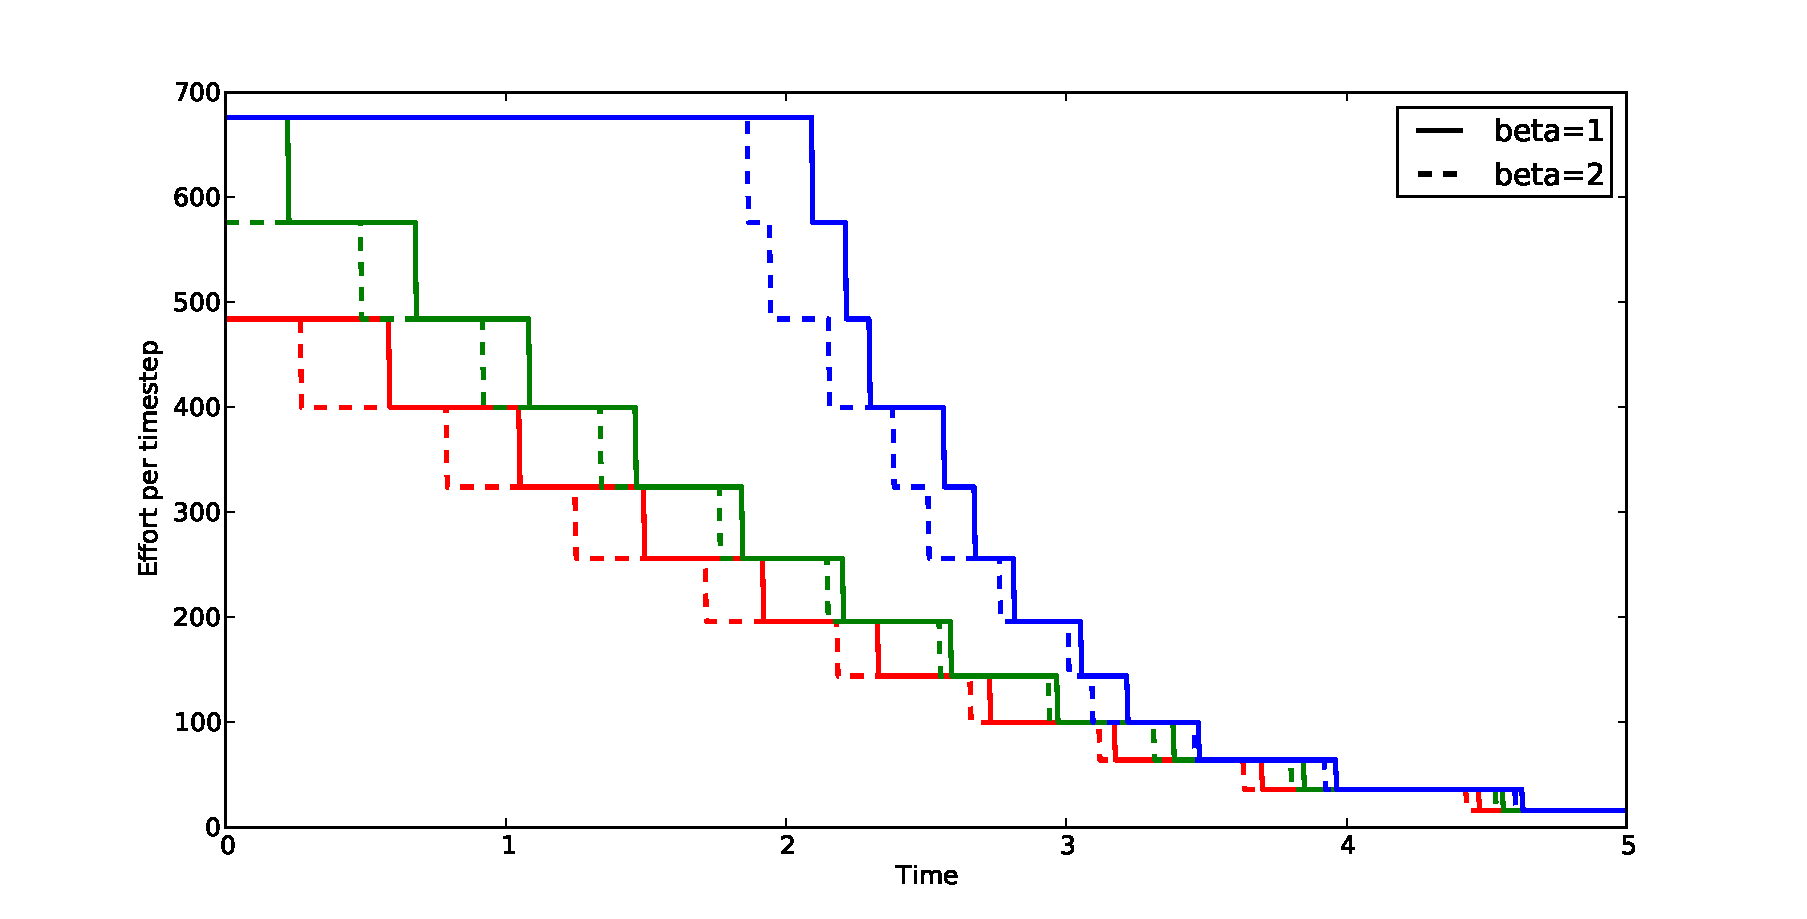
\includegraphics[width=11cm]{../figs/polboltz/adapt}
\end{frame}

\begin{frame}{NC: Polar}
\[
    f_0(\Bv) = \exp(-5|\Bv|^2) + \exp(-5(v_x-1)^2-12v_y^2),
\]
\centering
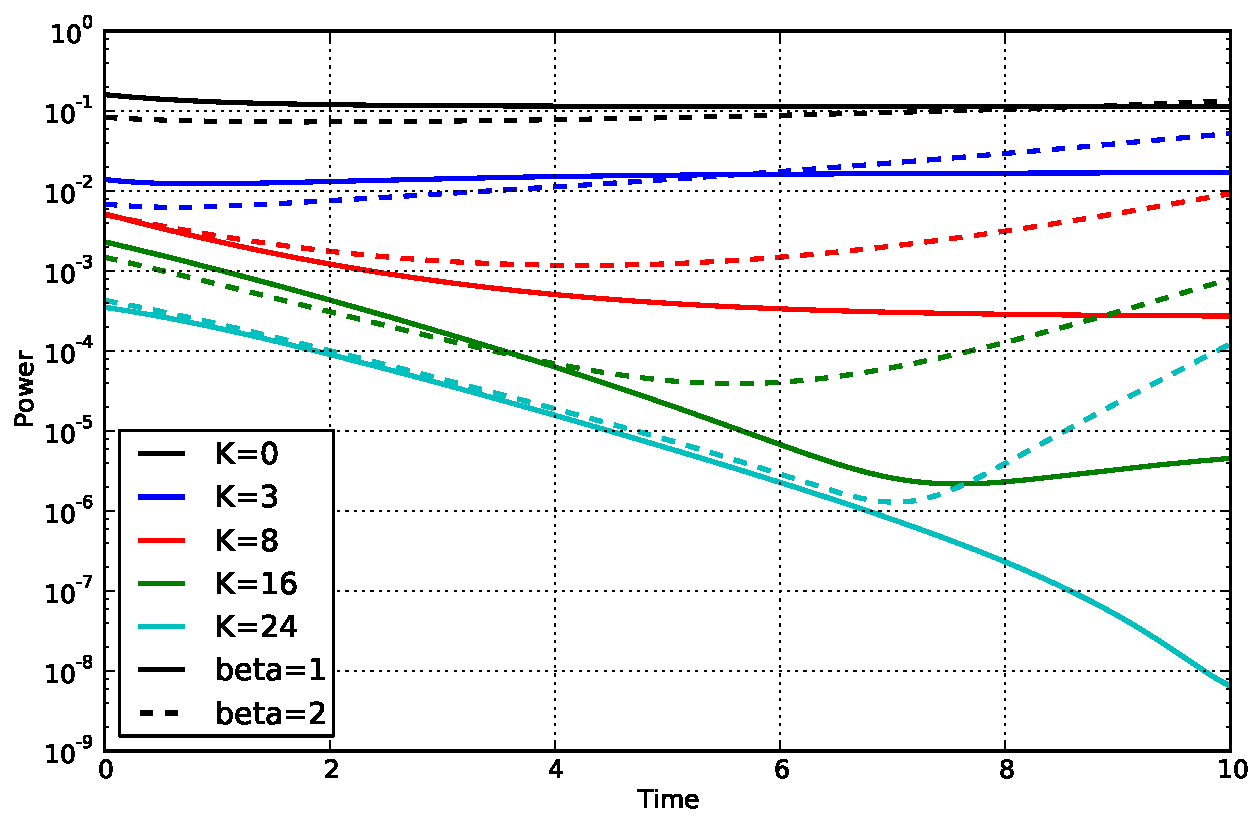
\includegraphics[width=8cm]{../figs/polboltz/power-comp2}
\end{frame}

\begin{frame}{Aliasing in Fourier method}
\centering
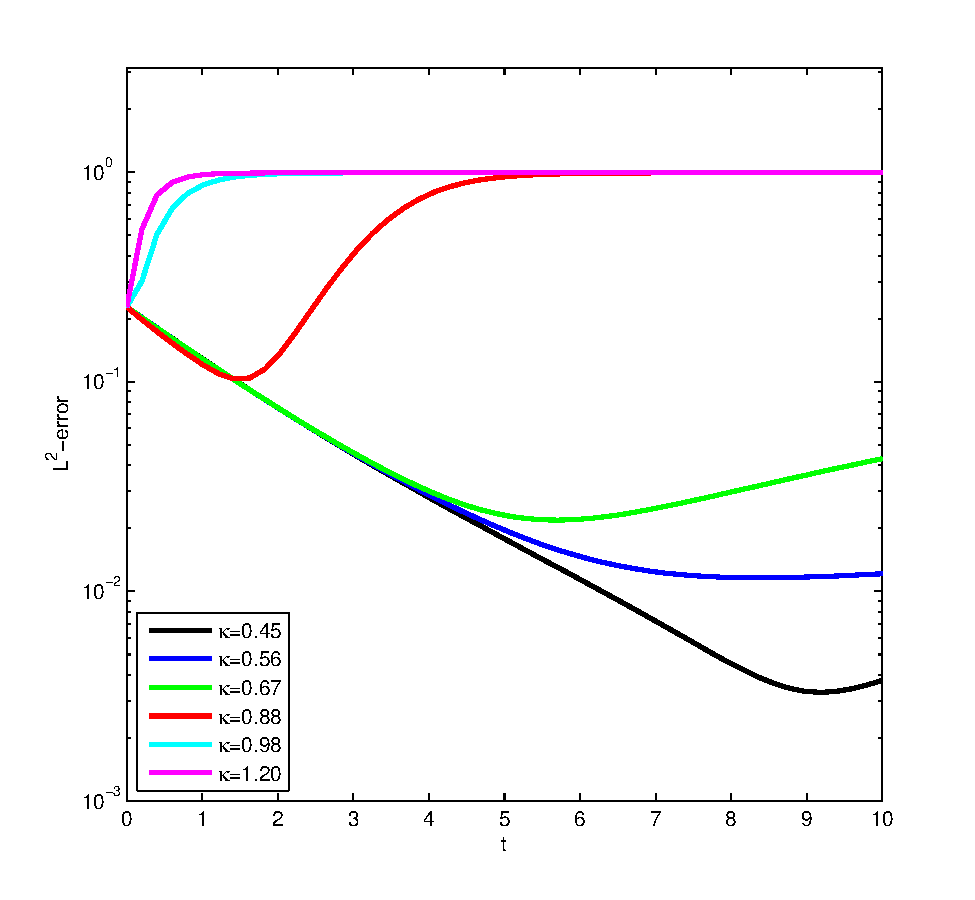
\includegraphics[width=7cm]{../figs/hcboltz/testr} \\
Error at various $\kappa$ for the BKW solution.
\end{frame}

\begin{frame}{BKW: Polar vs. Fourier}
\[
    f_0(\Bv) = 4 \exp(-2|\Bv|^2) |\Bv|^2
\]
$44\times26$ for polar, $80\times80$ for Fourier, using $L=\pi,\nicefrac{3\pi}{2},3\pi$. \\~\\

\centering
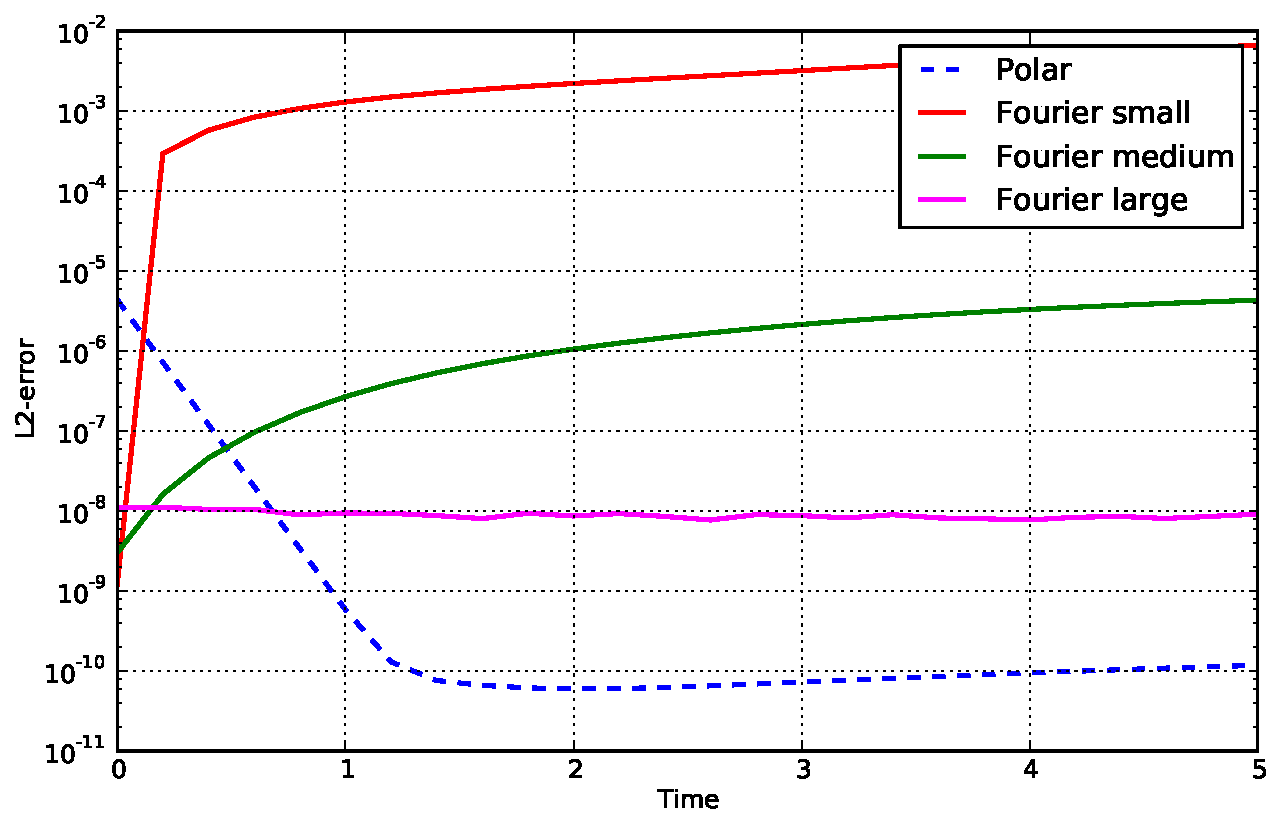
\includegraphics[width=8cm]{../figs/polboltz/compare-bkw}
\end{frame}

\begin{frame}{Summary}
\begin{itemize}[label=\ding{221}]
    \item HC Fourier can be good far from equilibrum
    \item Polar method is good near equilibrium (long times)
    \item Polar method is easily adaptive
    \item Polar method with $\beta=1$ is fully conservative
    \item Polar method suffers no aliasing
    \item Polar method appears to converge in time
\end{itemize}
\end{frame}

% \section*{Bibliography}
% \bibliographystyle{apalike}
% \bibliography{literatur} 

%\input{appendix.tex}
\end{document}
